% Options for packages loaded elsewhere
\PassOptionsToPackage{unicode}{hyperref}
\PassOptionsToPackage{hyphens}{url}
%
\documentclass[
]{article}
\usepackage{lmodern}
\usepackage{amssymb,amsmath}
\usepackage{ifxetex,ifluatex}
\ifnum 0\ifxetex 1\fi\ifluatex 1\fi=0 % if pdftex
  \usepackage[T1]{fontenc}
  \usepackage[utf8]{inputenc}
  \usepackage{textcomp} % provide euro and other symbols
\else % if luatex or xetex
  \usepackage{unicode-math}
  \defaultfontfeatures{Scale=MatchLowercase}
  \defaultfontfeatures[\rmfamily]{Ligatures=TeX,Scale=1}
\fi
% Use upquote if available, for straight quotes in verbatim environments
\IfFileExists{upquote.sty}{\usepackage{upquote}}{}
\IfFileExists{microtype.sty}{% use microtype if available
  \usepackage[]{microtype}
  \UseMicrotypeSet[protrusion]{basicmath} % disable protrusion for tt fonts
}{}
\makeatletter
\@ifundefined{KOMAClassName}{% if non-KOMA class
  \IfFileExists{parskip.sty}{%
    \usepackage{parskip}
  }{% else
    \setlength{\parindent}{0pt}
    \setlength{\parskip}{6pt plus 2pt minus 1pt}}
}{% if KOMA class
  \KOMAoptions{parskip=half}}
\makeatother
\usepackage{xcolor}
\IfFileExists{xurl.sty}{\usepackage{xurl}}{} % add URL line breaks if available
\IfFileExists{bookmark.sty}{\usepackage{bookmark}}{\usepackage{hyperref}}
\hypersetup{
  pdftitle={HW2\_Liu Zi Jian},
  pdfauthor={Zi Jian Liu},
  hidelinks,
  pdfcreator={LaTeX via pandoc}}
\urlstyle{same} % disable monospaced font for URLs
\usepackage[margin=1in]{geometry}
\usepackage{color}
\usepackage{fancyvrb}
\newcommand{\VerbBar}{|}
\newcommand{\VERB}{\Verb[commandchars=\\\{\}]}
\DefineVerbatimEnvironment{Highlighting}{Verbatim}{commandchars=\\\{\}}
% Add ',fontsize=\small' for more characters per line
\usepackage{framed}
\definecolor{shadecolor}{RGB}{248,248,248}
\newenvironment{Shaded}{\begin{snugshade}}{\end{snugshade}}
\newcommand{\AlertTok}[1]{\textcolor[rgb]{0.94,0.16,0.16}{#1}}
\newcommand{\AnnotationTok}[1]{\textcolor[rgb]{0.56,0.35,0.01}{\textbf{\textit{#1}}}}
\newcommand{\AttributeTok}[1]{\textcolor[rgb]{0.77,0.63,0.00}{#1}}
\newcommand{\BaseNTok}[1]{\textcolor[rgb]{0.00,0.00,0.81}{#1}}
\newcommand{\BuiltInTok}[1]{#1}
\newcommand{\CharTok}[1]{\textcolor[rgb]{0.31,0.60,0.02}{#1}}
\newcommand{\CommentTok}[1]{\textcolor[rgb]{0.56,0.35,0.01}{\textit{#1}}}
\newcommand{\CommentVarTok}[1]{\textcolor[rgb]{0.56,0.35,0.01}{\textbf{\textit{#1}}}}
\newcommand{\ConstantTok}[1]{\textcolor[rgb]{0.00,0.00,0.00}{#1}}
\newcommand{\ControlFlowTok}[1]{\textcolor[rgb]{0.13,0.29,0.53}{\textbf{#1}}}
\newcommand{\DataTypeTok}[1]{\textcolor[rgb]{0.13,0.29,0.53}{#1}}
\newcommand{\DecValTok}[1]{\textcolor[rgb]{0.00,0.00,0.81}{#1}}
\newcommand{\DocumentationTok}[1]{\textcolor[rgb]{0.56,0.35,0.01}{\textbf{\textit{#1}}}}
\newcommand{\ErrorTok}[1]{\textcolor[rgb]{0.64,0.00,0.00}{\textbf{#1}}}
\newcommand{\ExtensionTok}[1]{#1}
\newcommand{\FloatTok}[1]{\textcolor[rgb]{0.00,0.00,0.81}{#1}}
\newcommand{\FunctionTok}[1]{\textcolor[rgb]{0.00,0.00,0.00}{#1}}
\newcommand{\ImportTok}[1]{#1}
\newcommand{\InformationTok}[1]{\textcolor[rgb]{0.56,0.35,0.01}{\textbf{\textit{#1}}}}
\newcommand{\KeywordTok}[1]{\textcolor[rgb]{0.13,0.29,0.53}{\textbf{#1}}}
\newcommand{\NormalTok}[1]{#1}
\newcommand{\OperatorTok}[1]{\textcolor[rgb]{0.81,0.36,0.00}{\textbf{#1}}}
\newcommand{\OtherTok}[1]{\textcolor[rgb]{0.56,0.35,0.01}{#1}}
\newcommand{\PreprocessorTok}[1]{\textcolor[rgb]{0.56,0.35,0.01}{\textit{#1}}}
\newcommand{\RegionMarkerTok}[1]{#1}
\newcommand{\SpecialCharTok}[1]{\textcolor[rgb]{0.00,0.00,0.00}{#1}}
\newcommand{\SpecialStringTok}[1]{\textcolor[rgb]{0.31,0.60,0.02}{#1}}
\newcommand{\StringTok}[1]{\textcolor[rgb]{0.31,0.60,0.02}{#1}}
\newcommand{\VariableTok}[1]{\textcolor[rgb]{0.00,0.00,0.00}{#1}}
\newcommand{\VerbatimStringTok}[1]{\textcolor[rgb]{0.31,0.60,0.02}{#1}}
\newcommand{\WarningTok}[1]{\textcolor[rgb]{0.56,0.35,0.01}{\textbf{\textit{#1}}}}
\usepackage{graphicx,grffile}
\makeatletter
\def\maxwidth{\ifdim\Gin@nat@width>\linewidth\linewidth\else\Gin@nat@width\fi}
\def\maxheight{\ifdim\Gin@nat@height>\textheight\textheight\else\Gin@nat@height\fi}
\makeatother
% Scale images if necessary, so that they will not overflow the page
% margins by default, and it is still possible to overwrite the defaults
% using explicit options in \includegraphics[width, height, ...]{}
\setkeys{Gin}{width=\maxwidth,height=\maxheight,keepaspectratio}
% Set default figure placement to htbp
\makeatletter
\def\fps@figure{htbp}
\makeatother
\setlength{\emergencystretch}{3em} % prevent overfull lines
\providecommand{\tightlist}{%
  \setlength{\itemsep}{0pt}\setlength{\parskip}{0pt}}
\setcounter{secnumdepth}{-\maxdimen} % remove section numbering

\title{HW2\_Liu Zi Jian}
\author{Zi Jian Liu}
\date{05/02/2021}

\begin{document}
\maketitle

{
\setcounter{tocdepth}{2}
\tableofcontents
}
\hypertarget{question-1}{%
\section{Question 1}\label{question-1}}

\hypertarget{a}{%
\subsection{1 a)}\label{a}}

\begin{Shaded}
\begin{Highlighting}[]
\NormalTok{housingData <-}\StringTok{ }\KeywordTok{read.csv}\NormalTok{(}\StringTok{'_data_hw2/housingprice.csv'}\NormalTok{)}
\KeywordTok{head}\NormalTok{(housingData)}
\end{Highlighting}
\end{Shaded}

\begin{verbatim}
##           id            date   price bedrooms bathrooms sqft_living sqft_lot
## 1 7129300520 20141013T000000  221900        3      1.00        1180     5650
## 2 6414100192 20141209T000000  538000        3      2.25        2570     7242
## 3 5631500400 20150225T000000  180000        2      1.00         770    10000
## 4 2487200875 20141209T000000  604000        4      3.00        1960     5000
## 5 1954400510 20150218T000000  510000        3      2.00        1680     8080
## 6 7237550310 20140512T000000 1225000        4      4.50        5420   101930
##   floors waterfront view condition grade sqft_above sqft_basement yr_built
## 1      1          0    0         3     7       1180             0     1955
## 2      2          0    0         3     7       2170           400     1951
## 3      1          0    0         3     6        770             0     1933
## 4      1          0    0         5     7       1050           910     1965
## 5      1          0    0         3     8       1680             0     1987
## 6      1          0    0         3    11       3890          1530     2001
##   yr_renovated zipcode     lat     long sqft_living15 sqft_lot15
## 1            0   98178 47.5112 -122.257          1340       5650
## 2         1991   98125 47.7210 -122.319          1690       7639
## 3            0   98028 47.7379 -122.233          2720       8062
## 4            0   98136 47.5208 -122.393          1360       5000
## 5            0   98074 47.6168 -122.045          1800       7503
## 6            0   98053 47.6561 -122.005          4760     101930
\end{verbatim}

\begin{Shaded}
\begin{Highlighting}[]
\CommentTok{# coverting zipcode column into factors}
\NormalTok{housingData}\OperatorTok{$}\NormalTok{zipcode <-}\StringTok{ }\KeywordTok{as.factor}\NormalTok{(housingData}\OperatorTok{$}\NormalTok{zipcode)}
\end{Highlighting}
\end{Shaded}

Finding the most expensive zipcodes:

\begin{Shaded}
\begin{Highlighting}[]
\NormalTok{avgPrice <-}\StringTok{ }\KeywordTok{tapply}\NormalTok{(housingData}\OperatorTok{$}\NormalTok{price, housingData}\OperatorTok{$}\NormalTok{zipcode, mean)}
\NormalTok{avgPrice <-}\StringTok{ }\KeywordTok{sort}\NormalTok{(avgPrice, }\DataTypeTok{decreasing =} \OtherTok{TRUE}\NormalTok{)}
\NormalTok{avgPrice[}\DecValTok{1}\OperatorTok{:}\DecValTok{3}\NormalTok{]}
\end{Highlighting}
\end{Shaded}

\begin{verbatim}
##   98039   98004   98040 
## 2160607 1355927 1194230
\end{verbatim}

The top 3 zipcodes whose housing prices are the most expensive is 98039,
98004, and 98040

Boxplots of housing prices for these 3 zipcodes:

\begin{Shaded}
\begin{Highlighting}[]
\NormalTok{plot1 =}\StringTok{ }\KeywordTok{subset}\NormalTok{(housingData, zipcode }\OperatorTok{==}\StringTok{ }\DecValTok{98039}\NormalTok{, }\DataTypeTok{select =} \KeywordTok{c}\NormalTok{(price))}
\NormalTok{plot2 =}\StringTok{ }\KeywordTok{subset}\NormalTok{(housingData, zipcode }\OperatorTok{==}\StringTok{ }\DecValTok{98004}\NormalTok{, }\DataTypeTok{select =} \KeywordTok{c}\NormalTok{(price))}
\NormalTok{plot3 =}\StringTok{ }\KeywordTok{subset}\NormalTok{(housingData, zipcode }\OperatorTok{==}\StringTok{ }\DecValTok{98040}\NormalTok{, }\DataTypeTok{select =} \KeywordTok{c}\NormalTok{(price))}

\KeywordTok{boxplot}\NormalTok{(plot1)}
\end{Highlighting}
\end{Shaded}

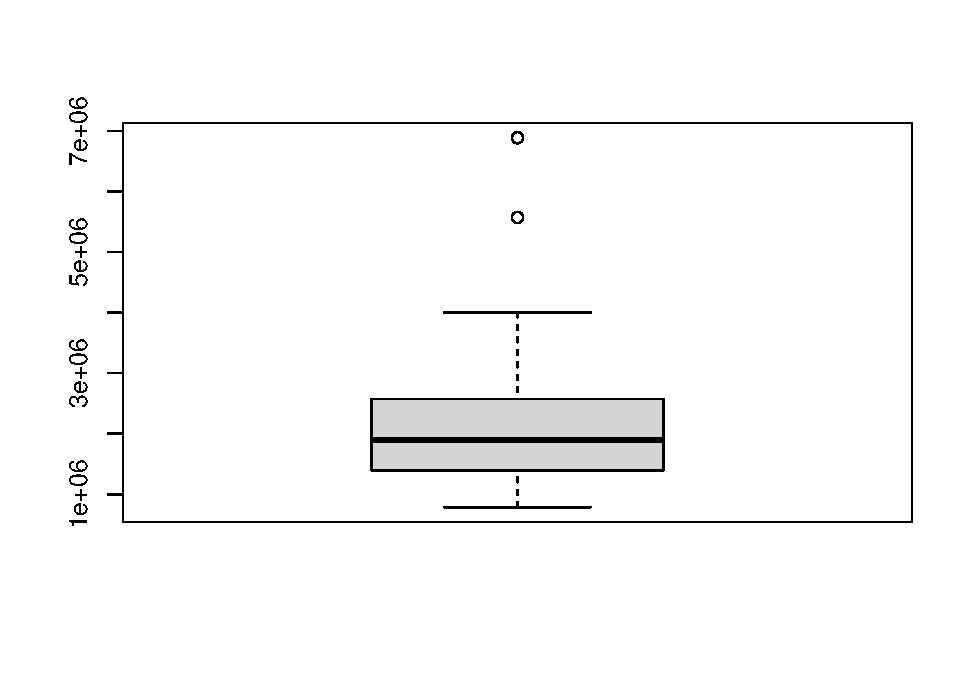
\includegraphics{HW2_Liu-Zi-Jian_files/figure-latex/unnamed-chunk-3-1.pdf}

\begin{Shaded}
\begin{Highlighting}[]
\KeywordTok{boxplot}\NormalTok{(plot2)}
\end{Highlighting}
\end{Shaded}

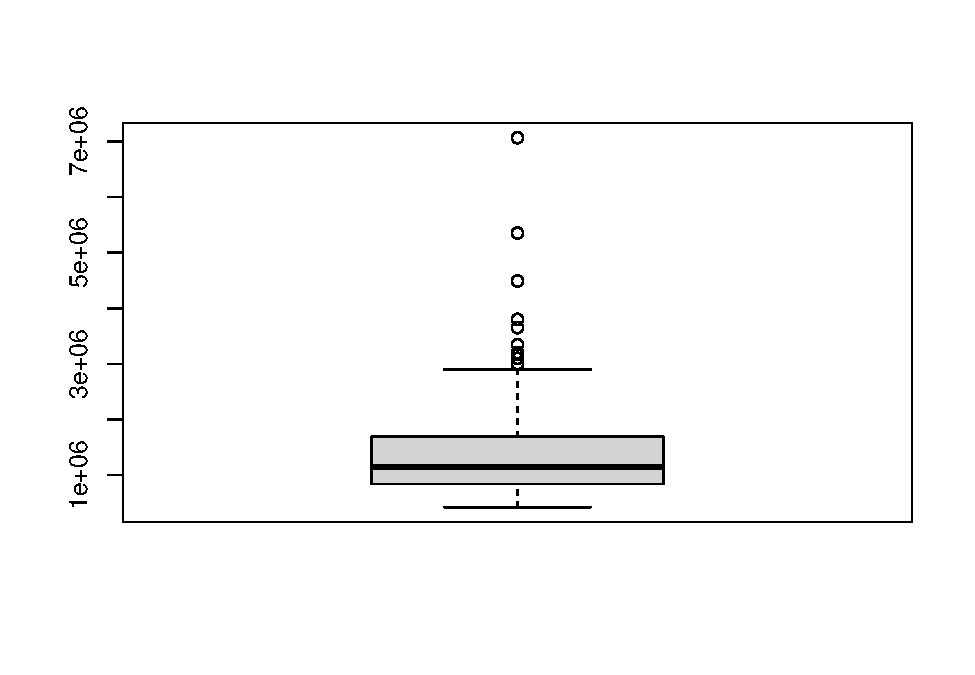
\includegraphics{HW2_Liu-Zi-Jian_files/figure-latex/unnamed-chunk-3-2.pdf}

\begin{Shaded}
\begin{Highlighting}[]
\KeywordTok{boxplot}\NormalTok{(plot3)}
\end{Highlighting}
\end{Shaded}

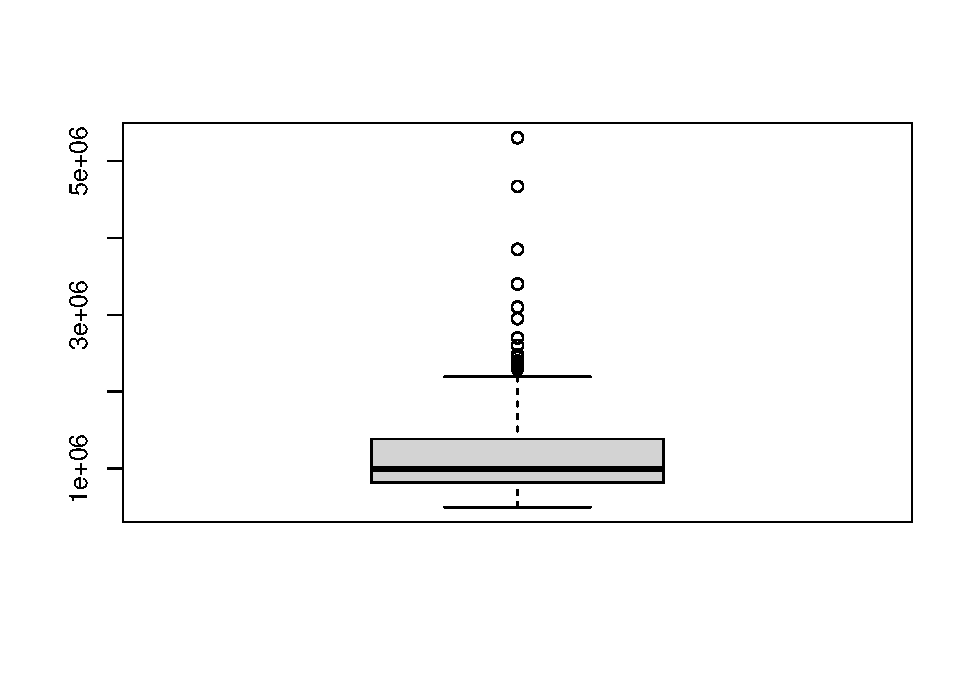
\includegraphics{HW2_Liu-Zi-Jian_files/figure-latex/unnamed-chunk-3-3.pdf}

Above is the boxplots of the housing prices for the most expensive 3
zipcodes.

\hypertarget{b.-scatter-plot}{%
\subsection{1 b). Scatter plot}\label{b.-scatter-plot}}

\begin{Shaded}
\begin{Highlighting}[]
\KeywordTok{plot}\NormalTok{(housingData}\OperatorTok{$}\NormalTok{sqft_living, housingData}\OperatorTok{$}\NormalTok{price, }\DataTypeTok{main=}\StringTok{"relationship between sqft and price"}\NormalTok{,}
   \DataTypeTok{xlab=}\StringTok{"sqft living"}\NormalTok{, }\DataTypeTok{ylab=}\StringTok{"price"}\NormalTok{, }\DataTypeTok{pch=}\DecValTok{20}\NormalTok{)}
\end{Highlighting}
\end{Shaded}

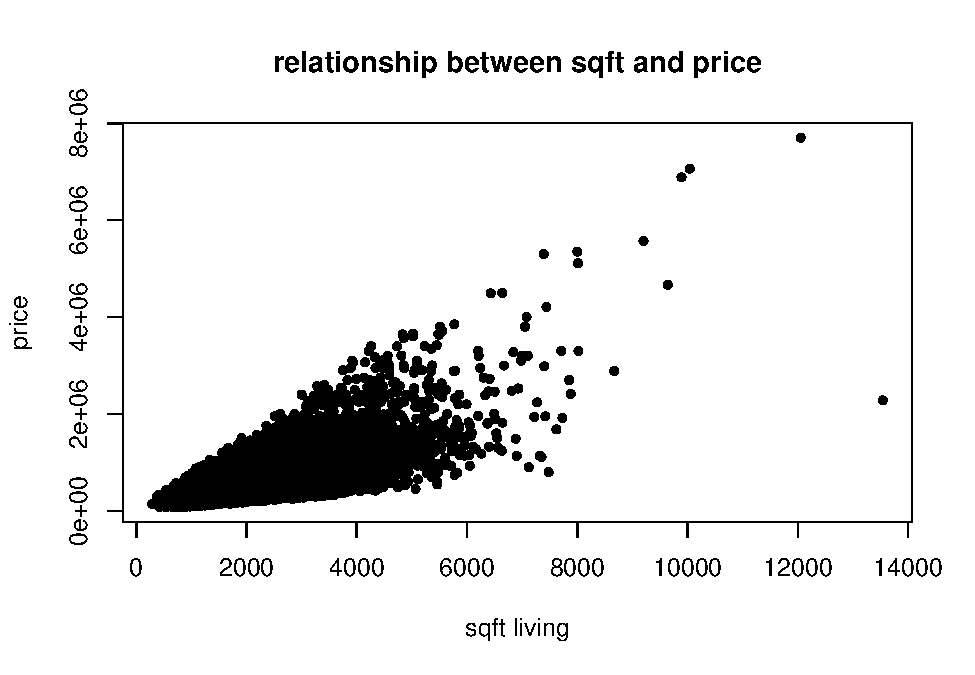
\includegraphics{HW2_Liu-Zi-Jian_files/figure-latex/unnamed-chunk-4-1.pdf}

above is a scatterplot showing the relationship between sqft and price.

\hypertarget{c.}{%
\subsection{1 c).}\label{c.}}

\begin{Shaded}
\begin{Highlighting}[]
\NormalTok{train =}\StringTok{ }\KeywordTok{read.csv}\NormalTok{(}\StringTok{'_data_hw2/train.data.csv'}\NormalTok{)}
\KeywordTok{head}\NormalTok{(train)}
\end{Highlighting}
\end{Shaded}

\begin{verbatim}
##   X         id            date   price bedrooms bathrooms sqft_living sqft_lot
## 1 2 6414100192 20141209T000000  538000        3      2.25        2570     7242
## 2 4 2487200875 20141209T000000  604000        4      3.00        1960     5000
## 3 5 1954400510 20150218T000000  510000        3      2.00        1680     8080
## 4 6 7237550310 20140512T000000 1225000        4      4.50        5420   101930
## 5 7 1321400060 20140627T000000  257500        3      2.25        1715     6819
## 6 8 2008000270 20150115T000000  291850        3      1.50        1060     9711
##   floors waterfront view condition grade sqft_above sqft_basement yr_built
## 1      2          0    0         3     7       2170           400     1951
## 2      1          0    0         5     7       1050           910     1965
## 3      1          0    0         3     8       1680             0     1987
## 4      1          0    0         3    11       3890          1530     2001
## 5      2          0    0         3     7       1715             0     1995
## 6      1          0    0         3     7       1060             0     1963
##   yr_renovated zipcode     lat     long sqft_living15 sqft_lot15
## 1         1991   98125 47.7210 -122.319          1690       7639
## 2            0   98136 47.5208 -122.393          1360       5000
## 3            0   98074 47.6168 -122.045          1800       7503
## 4            0   98053 47.6561 -122.005          4760     101930
## 5            0   98003 47.3097 -122.327          2238       6819
## 6            0   98198 47.4095 -122.315          1650       9711
\end{verbatim}

\begin{Shaded}
\begin{Highlighting}[]
\NormalTok{test =}\StringTok{ }\KeywordTok{read.csv}\NormalTok{(}\StringTok{'_data_hw2/test.data.csv'}\NormalTok{)}
\KeywordTok{head}\NormalTok{(test)}
\end{Highlighting}
\end{Shaded}

\begin{verbatim}
##    X         id            date  price bedrooms bathrooms sqft_living sqft_lot
## 1  1 7129300520 20141013T000000 221900        3       1.0        1180     5650
## 2  3 5631500400 20150225T000000 180000        2       1.0         770    10000
## 3 11 1736800520 20150403T000000 662500        3       2.5        3560     9796
## 4 18 6865200140 20140529T000000 485000        4       1.0        1600     4300
## 5 20 7983200060 20150424T000000 230000        3       1.0        1250     9774
## 6 24 8091400200 20140516T000000 252700        2       1.5        1070     9643
##   floors waterfront view condition grade sqft_above sqft_basement yr_built
## 1    1.0          0    0         3     7       1180             0     1955
## 2    1.0          0    0         3     6        770             0     1933
## 3    1.0          0    0         3     8       1860          1700     1965
## 4    1.5          0    0         4     7       1600             0     1916
## 5    1.0          0    0         4     7       1250             0     1969
## 6    1.0          0    0         3     7       1070             0     1985
##   yr_renovated zipcode     lat     long sqft_living15 sqft_lot15
## 1            0   98178 47.5112 -122.257          1340       5650
## 2            0   98028 47.7379 -122.233          2720       8062
## 3            0   98007 47.6007 -122.145          2210       8925
## 4            0   98103 47.6648 -122.343          1610       4300
## 5            0   98003 47.3343 -122.306          1280       8850
## 6            0   98030 47.3533 -122.166          1220       8386
\end{verbatim}

\begin{Shaded}
\begin{Highlighting}[]
\CommentTok{# training}
\NormalTok{modelprice =}\StringTok{ }\KeywordTok{lm}\NormalTok{(price }\OperatorTok{~}\StringTok{ }\NormalTok{bedrooms }\OperatorTok{+}\StringTok{ }\NormalTok{bathrooms }\OperatorTok{+}\StringTok{ }\NormalTok{sqft_living }\OperatorTok{+}\StringTok{ }\NormalTok{sqft_lot, }\DataTypeTok{data =}\NormalTok{ train)}
\KeywordTok{summary}\NormalTok{(modelprice)}
\end{Highlighting}
\end{Shaded}

\begin{verbatim}
## 
## Call:
## lm(formula = price ~ bedrooms + bathrooms + sqft_living + sqft_lot, 
##     data = train)
## 
## Residuals:
##      Min       1Q   Median       3Q      Max 
## -1571803  -143678   -22595   103133  4141210 
## 
## Coefficients:
##               Estimate Std. Error t value Pr(>|t|)    
## (Intercept)  8.083e+04  8.208e+03   9.848  < 2e-16 ***
## bedrooms    -5.930e+04  2.753e+03 -21.537  < 2e-16 ***
## bathrooms    3.682e+03  4.178e+03   0.881    0.378    
## sqft_living  3.167e+02  3.750e+00  84.442  < 2e-16 ***
## sqft_lot    -4.267e-01  5.504e-02  -7.753 9.52e-15 ***
## ---
## Signif. codes:  0 '***' 0.001 '**' 0.01 '*' 0.05 '.' 0.1 ' ' 1
## 
## Residual standard error: 257200 on 15124 degrees of freedom
## Multiple R-squared:  0.5101, Adjusted R-squared:   0.51 
## F-statistic:  3937 on 4 and 15124 DF,  p-value: < 2.2e-16
\end{verbatim}

The Rsquared of the model on training data is 0.5101

\begin{Shaded}
\begin{Highlighting}[]
\CommentTok{# Evaluate model on test data}
\NormalTok{testpredict =}\StringTok{ }\KeywordTok{predict}\NormalTok{(modelprice, test)}
\NormalTok{prices =}\StringTok{ }\NormalTok{test}\OperatorTok{$}\NormalTok{price}
\NormalTok{e =}\StringTok{ }\NormalTok{prices }\OperatorTok{-}\StringTok{ }\NormalTok{testpredict}
\NormalTok{R2 =}\StringTok{ }\DecValTok{1}\OperatorTok{-}\KeywordTok{sum}\NormalTok{(e}\OperatorTok{^}\DecValTok{2}\NormalTok{)}\OperatorTok{/}\KeywordTok{sum}\NormalTok{((prices}\OperatorTok{-}\KeywordTok{mean}\NormalTok{(prices))}\OperatorTok{^}\DecValTok{2}\NormalTok{)}
\NormalTok{R2}
\end{Highlighting}
\end{Shaded}

\begin{verbatim}
## [1] 0.5049945
\end{verbatim}

The Rsquared of the model on testing data is 0.505

\hypertarget{d-adding-zipcode}{%
\subsection{1. d) adding zipcode}\label{d-adding-zipcode}}

\begin{Shaded}
\begin{Highlighting}[]
\CommentTok{# training}
\NormalTok{modelpricezip =}\StringTok{ }\KeywordTok{lm}\NormalTok{(price }\OperatorTok{~}\StringTok{ }\NormalTok{bedrooms }\OperatorTok{+}\StringTok{ }\NormalTok{bathrooms }\OperatorTok{+}\StringTok{ }\NormalTok{sqft_living }\OperatorTok{+}\StringTok{ }\NormalTok{sqft_lot }\OperatorTok{+}\NormalTok{zipcode, }\DataTypeTok{data =}\NormalTok{ train)}
\KeywordTok{summary}\NormalTok{(modelpricezip)}
\end{Highlighting}
\end{Shaded}

\begin{verbatim}
## 
## Call:
## lm(formula = price ~ bedrooms + bathrooms + sqft_living + sqft_lot + 
##     zipcode, data = train)
## 
## Residuals:
##      Min       1Q   Median       3Q      Max 
## -1638518  -141274   -22673   101293  4074728 
## 
## Coefficients:
##               Estimate Std. Error t value Pr(>|t|)    
## (Intercept) -5.460e+07  3.933e+06 -13.883  < 2e-16 ***
## bedrooms    -5.760e+04  2.739e+03 -21.034  < 2e-16 ***
## bathrooms    8.631e+03  4.167e+03   2.071   0.0383 *  
## sqft_living  3.185e+02  3.729e+00  85.420  < 2e-16 ***
## sqft_lot    -3.443e-01  5.501e-02  -6.259 3.98e-10 ***
## zipcode      5.573e+02  4.008e+01  13.904  < 2e-16 ***
## ---
## Signif. codes:  0 '***' 0.001 '**' 0.01 '*' 0.05 '.' 0.1 ' ' 1
## 
## Residual standard error: 255600 on 15123 degrees of freedom
## Multiple R-squared:  0.5163, Adjusted R-squared:  0.5161 
## F-statistic:  3228 on 5 and 15123 DF,  p-value: < 2.2e-16
\end{verbatim}

The Rsquared of the model on training data is 0.5163

\begin{Shaded}
\begin{Highlighting}[]
\CommentTok{# Evaluate model on test data}
\NormalTok{testpredictzip =}\StringTok{ }\KeywordTok{predict}\NormalTok{(modelpricezip, test)}
\NormalTok{prices =}\StringTok{ }\NormalTok{test}\OperatorTok{$}\NormalTok{price}
\NormalTok{e =}\StringTok{ }\NormalTok{prices }\OperatorTok{-}\StringTok{ }\NormalTok{testpredictzip}
\NormalTok{R2zip =}\StringTok{ }\DecValTok{1}\OperatorTok{-}\KeywordTok{sum}\NormalTok{(e}\OperatorTok{^}\DecValTok{2}\NormalTok{)}\OperatorTok{/}\KeywordTok{sum}\NormalTok{((prices}\OperatorTok{-}\KeywordTok{mean}\NormalTok{(prices))}\OperatorTok{^}\DecValTok{2}\NormalTok{)}
\NormalTok{R2zip}
\end{Highlighting}
\end{Shaded}

\begin{verbatim}
## [1] 0.5120097
\end{verbatim}

The Rsquared of the model on testing data is 0.512

\hypertarget{e}{%
\subsection{1. e)}\label{e}}

\begin{Shaded}
\begin{Highlighting}[]
\NormalTok{fancy =}\StringTok{ }\KeywordTok{read.csv}\NormalTok{(}\StringTok{'_data_hw2/fancyhouse.csv'}\NormalTok{)}
\KeywordTok{head}\NormalTok{(fancy)}
\end{Highlighting}
\end{Shaded}

\begin{verbatim}
##   X bedrooms bathrooms sqft_living sqft_lot floors zipcode condition grade
## 1 1        8        25       50000   225000      4   98039        10    10
##   waterfront view sqft_above sqft_basement yr_built yr_renovated      lat
## 1          1    4      37500         12500     1994         2010 47.62761
##        long sqft_living15 sqft_lot15
## 1 -122.2421          5000      40000
\end{verbatim}

\begin{Shaded}
\begin{Highlighting}[]
\NormalTok{billgate =}\StringTok{ }\KeywordTok{predict}\NormalTok{(modelpricezip, fancy)}
\NormalTok{billgate}
\end{Highlighting}
\end{Shaded}

\begin{verbatim}
##        1 
## 15642273
\end{verbatim}

We predict that the price of bill gates house is 15,642,273. This is a
reasonable estimate for the price.

\hypertarget{f}{%
\subsection{1. f)}\label{f}}

\begin{Shaded}
\begin{Highlighting}[]
\NormalTok{n =}\StringTok{ }\KeywordTok{nrow}\NormalTok{(train)}
\NormalTok{d =}\StringTok{ }\KeywordTok{length}\NormalTok{(train)}
\NormalTok{n}
\end{Highlighting}
\end{Shaded}

\begin{verbatim}
## [1] 15129
\end{verbatim}

\begin{Shaded}
\begin{Highlighting}[]
\NormalTok{d}
\end{Highlighting}
\end{Shaded}

\begin{verbatim}
## [1] 22
\end{verbatim}

if n\textgreater d+1 (15129 \textgreater{} 22 + 1) then adding another
covariate never hurts R2 over the training data.

\begin{Shaded}
\begin{Highlighting}[]
\NormalTok{covariate4 =}\StringTok{ }\KeywordTok{lm}\NormalTok{(price }\OperatorTok{~}\StringTok{ }\NormalTok{bedrooms }\OperatorTok{+}\StringTok{ }\NormalTok{bathrooms }\OperatorTok{+}\StringTok{ }\NormalTok{sqft_living }\OperatorTok{+}\StringTok{ }\NormalTok{sqft_lot, }\DataTypeTok{data =}\NormalTok{ train)}
\NormalTok{covariate5 =}\StringTok{ }\KeywordTok{lm}\NormalTok{(price }\OperatorTok{~}\StringTok{ }\NormalTok{bedrooms }\OperatorTok{+}\StringTok{ }\NormalTok{bathrooms }\OperatorTok{+}\StringTok{ }\NormalTok{sqft_living }\OperatorTok{+}\StringTok{ }\NormalTok{sqft_lot }\OperatorTok{+}\StringTok{ }\NormalTok{zipcode, }\DataTypeTok{data =}\NormalTok{ train)}
\NormalTok{covariate6 =}\StringTok{ }\KeywordTok{lm}\NormalTok{(price }\OperatorTok{~}\StringTok{ }\NormalTok{bedrooms }\OperatorTok{+}\StringTok{ }\NormalTok{bathrooms }\OperatorTok{+}\StringTok{ }\NormalTok{sqft_living }\OperatorTok{+}\StringTok{ }\NormalTok{sqft_lot }\OperatorTok{+}\StringTok{ }\NormalTok{zipcode }\OperatorTok{+}\StringTok{ }\NormalTok{floors, }\DataTypeTok{data =}\NormalTok{ train)}
\NormalTok{covariate7 =}\StringTok{ }\KeywordTok{lm}\NormalTok{(price }\OperatorTok{~}\StringTok{ }\NormalTok{bedrooms }\OperatorTok{+}\StringTok{ }\NormalTok{bathrooms }\OperatorTok{+}\StringTok{ }\NormalTok{sqft_living }\OperatorTok{+}\StringTok{ }\NormalTok{sqft_lot }\OperatorTok{+}\StringTok{ }\NormalTok{zipcode }\OperatorTok{+}\StringTok{ }\NormalTok{floors }\OperatorTok{+}\StringTok{ }\NormalTok{condition, }\DataTypeTok{data =}\NormalTok{ train)}
\NormalTok{covariate8 =}\StringTok{ }\KeywordTok{lm}\NormalTok{(price }\OperatorTok{~}\StringTok{ }\NormalTok{bedrooms }\OperatorTok{+}\StringTok{ }\NormalTok{bathrooms }\OperatorTok{+}\StringTok{ }\NormalTok{sqft_living }\OperatorTok{+}\StringTok{ }\NormalTok{sqft_lot }\OperatorTok{+}\StringTok{ }\NormalTok{zipcode }\OperatorTok{+}\StringTok{ }\NormalTok{floors }\OperatorTok{+}\StringTok{ }\NormalTok{condition }\OperatorTok{+}\StringTok{ }\NormalTok{grade, }\DataTypeTok{data =}\NormalTok{ train)}
\KeywordTok{summary}\NormalTok{(covariate4)}
\end{Highlighting}
\end{Shaded}

\begin{verbatim}
## 
## Call:
## lm(formula = price ~ bedrooms + bathrooms + sqft_living + sqft_lot, 
##     data = train)
## 
## Residuals:
##      Min       1Q   Median       3Q      Max 
## -1571803  -143678   -22595   103133  4141210 
## 
## Coefficients:
##               Estimate Std. Error t value Pr(>|t|)    
## (Intercept)  8.083e+04  8.208e+03   9.848  < 2e-16 ***
## bedrooms    -5.930e+04  2.753e+03 -21.537  < 2e-16 ***
## bathrooms    3.682e+03  4.178e+03   0.881    0.378    
## sqft_living  3.167e+02  3.750e+00  84.442  < 2e-16 ***
## sqft_lot    -4.267e-01  5.504e-02  -7.753 9.52e-15 ***
## ---
## Signif. codes:  0 '***' 0.001 '**' 0.01 '*' 0.05 '.' 0.1 ' ' 1
## 
## Residual standard error: 257200 on 15124 degrees of freedom
## Multiple R-squared:  0.5101, Adjusted R-squared:   0.51 
## F-statistic:  3937 on 4 and 15124 DF,  p-value: < 2.2e-16
\end{verbatim}

\begin{Shaded}
\begin{Highlighting}[]
\KeywordTok{summary}\NormalTok{(covariate5)}
\end{Highlighting}
\end{Shaded}

\begin{verbatim}
## 
## Call:
## lm(formula = price ~ bedrooms + bathrooms + sqft_living + sqft_lot + 
##     zipcode, data = train)
## 
## Residuals:
##      Min       1Q   Median       3Q      Max 
## -1638518  -141274   -22673   101293  4074728 
## 
## Coefficients:
##               Estimate Std. Error t value Pr(>|t|)    
## (Intercept) -5.460e+07  3.933e+06 -13.883  < 2e-16 ***
## bedrooms    -5.760e+04  2.739e+03 -21.034  < 2e-16 ***
## bathrooms    8.631e+03  4.167e+03   2.071   0.0383 *  
## sqft_living  3.185e+02  3.729e+00  85.420  < 2e-16 ***
## sqft_lot    -3.443e-01  5.501e-02  -6.259 3.98e-10 ***
## zipcode      5.573e+02  4.008e+01  13.904  < 2e-16 ***
## ---
## Signif. codes:  0 '***' 0.001 '**' 0.01 '*' 0.05 '.' 0.1 ' ' 1
## 
## Residual standard error: 255600 on 15123 degrees of freedom
## Multiple R-squared:  0.5163, Adjusted R-squared:  0.5161 
## F-statistic:  3228 on 5 and 15123 DF,  p-value: < 2.2e-16
\end{verbatim}

\begin{Shaded}
\begin{Highlighting}[]
\KeywordTok{summary}\NormalTok{(covariate6)}
\end{Highlighting}
\end{Shaded}

\begin{verbatim}
## 
## Call:
## lm(formula = price ~ bedrooms + bathrooms + sqft_living + sqft_lot + 
##     zipcode + floors, data = train)
## 
## Residuals:
##      Min       1Q   Median       3Q      Max 
## -1640835  -140857   -22328   101254  4068220 
## 
## Coefficients:
##               Estimate Std. Error t value Pr(>|t|)    
## (Intercept) -5.479e+07  3.936e+06 -13.920  < 2e-16 ***
## bedrooms    -5.797e+04  2.755e+03 -21.038  < 2e-16 ***
## bathrooms    1.074e+04  4.523e+03   2.374   0.0176 *  
## sqft_living  3.186e+02  3.729e+00  85.429  < 2e-16 ***
## sqft_lot    -3.483e-01  5.511e-02  -6.320 2.69e-10 ***
## zipcode      5.593e+02  4.012e+01  13.942  < 2e-16 ***
## floors      -5.377e+03  4.492e+03  -1.197   0.2313    
## ---
## Signif. codes:  0 '***' 0.001 '**' 0.01 '*' 0.05 '.' 0.1 ' ' 1
## 
## Residual standard error: 255600 on 15122 degrees of freedom
## Multiple R-squared:  0.5163, Adjusted R-squared:  0.5162 
## F-statistic:  2691 on 6 and 15122 DF,  p-value: < 2.2e-16
\end{verbatim}

\begin{Shaded}
\begin{Highlighting}[]
\KeywordTok{summary}\NormalTok{(covariate7)}
\end{Highlighting}
\end{Shaded}

\begin{verbatim}
## 
## Call:
## lm(formula = price ~ bedrooms + bathrooms + sqft_living + sqft_lot + 
##     zipcode + floors + condition, data = train)
## 
## Residuals:
##      Min       1Q   Median       3Q      Max 
## -1640138  -140116   -22533   100695  4023537 
## 
## Coefficients:
##               Estimate Std. Error t value Pr(>|t|)    
## (Intercept) -5.584e+07  3.904e+06 -14.301  < 2e-16 ***
## bedrooms    -6.131e+04  2.741e+03 -22.368  < 2e-16 ***
## bathrooms    1.355e+04  4.489e+03   3.018  0.00255 ** 
## sqft_living  3.175e+02  3.699e+00  85.812  < 2e-16 ***
## sqft_lot    -3.340e-01  5.467e-02  -6.109 1.03e-09 ***
## zipcode      5.680e+02  3.979e+01  14.273  < 2e-16 ***
## floors       1.138e+04  4.578e+03   2.485  0.01295 *  
## condition    5.233e+04  3.299e+03  15.863  < 2e-16 ***
## ---
## Signif. codes:  0 '***' 0.001 '**' 0.01 '*' 0.05 '.' 0.1 ' ' 1
## 
## Residual standard error: 253500 on 15121 degrees of freedom
## Multiple R-squared:  0.5243, Adjusted R-squared:  0.524 
## F-statistic:  2380 on 7 and 15121 DF,  p-value: < 2.2e-16
\end{verbatim}

\begin{Shaded}
\begin{Highlighting}[]
\KeywordTok{summary}\NormalTok{(covariate8)}
\end{Highlighting}
\end{Shaded}

\begin{verbatim}
## 
## Call:
## lm(formula = price ~ bedrooms + bathrooms + sqft_living + sqft_lot + 
##     zipcode + floors + condition + grade, data = train)
## 
## Residuals:
##      Min       1Q   Median       3Q      Max 
## -1133407  -129490   -20549    93466  4477104 
## 
## Coefficients:
##               Estimate Std. Error t value Pr(>|t|)    
## (Intercept) -6.404e+07  3.742e+06 -17.111  < 2e-16 ***
## bedrooms    -4.436e+04  2.662e+03 -16.664  < 2e-16 ***
## bathrooms   -6.287e+03  4.329e+03  -1.452    0.146    
## sqft_living  2.259e+02  4.306e+00  52.448  < 2e-16 ***
## sqft_lot    -2.770e-01  5.233e-02  -5.292 1.22e-07 ***
## zipcode      6.454e+02  3.813e+01  16.925  < 2e-16 ***
## floors      -2.602e+04  4.494e+03  -5.791 7.14e-09 ***
## condition    6.067e+04  3.164e+03  19.175  < 2e-16 ***
## grade        1.053e+05  2.819e+03  37.353  < 2e-16 ***
## ---
## Signif. codes:  0 '***' 0.001 '**' 0.01 '*' 0.05 '.' 0.1 ' ' 1
## 
## Residual standard error: 242600 on 15120 degrees of freedom
## Multiple R-squared:  0.5645, Adjusted R-squared:  0.5642 
## F-statistic:  2449 on 8 and 15120 DF,  p-value: < 2.2e-16
\end{verbatim}

As we can see above, adding another covariate to our model either does
not change our Rsquared or increases our Rsquared.

\hypertarget{question-2.}{%
\section{Question 2.}\label{question-2.}}

\hypertarget{a.}{%
\subsection{2 a).}\label{a.}}

\begin{Shaded}
\begin{Highlighting}[]
\NormalTok{modelmult =}\StringTok{ }\KeywordTok{lm}\NormalTok{(price }\OperatorTok{~}\StringTok{ }\NormalTok{bedrooms }\OperatorTok{+}\StringTok{ }\NormalTok{bathrooms }\OperatorTok{+}\StringTok{ }\NormalTok{sqft_living }\OperatorTok{+}\StringTok{ }\NormalTok{sqft_lot }\OperatorTok{+}\StringTok{ }\NormalTok{zipcode }\OperatorTok{+}\StringTok{ }\NormalTok{bedrooms }\OperatorTok{*}\StringTok{ }\NormalTok{bathrooms, }\DataTypeTok{data =}\NormalTok{ train)}
\KeywordTok{summary}\NormalTok{(modelmult)}
\end{Highlighting}
\end{Shaded}

\begin{verbatim}
## 
## Call:
## lm(formula = price ~ bedrooms + bathrooms + sqft_living + sqft_lot + 
##     zipcode + bedrooms * bathrooms, data = train)
## 
## Residuals:
##      Min       1Q   Median       3Q      Max 
## -2202454  -139444   -23520   100249  3685052 
## 
## Coefficients:
##                      Estimate Std. Error t value Pr(>|t|)    
## (Intercept)        -4.920e+07  3.928e+06 -12.526  < 2e-16 ***
## bedrooms           -1.216e+05  5.359e+03 -22.697  < 2e-16 ***
## bathrooms          -9.739e+04  8.694e+03 -11.203  < 2e-16 ***
## sqft_living         3.110e+02  3.745e+00  83.054  < 2e-16 ***
## sqft_lot           -3.502e-01  5.467e-02  -6.405 1.55e-10 ***
## zipcode             5.045e+02  4.001e+01  12.608  < 2e-16 ***
## bedrooms:bathrooms  3.107e+04  2.240e+03  13.871  < 2e-16 ***
## ---
## Signif. codes:  0 '***' 0.001 '**' 0.01 '*' 0.05 '.' 0.1 ' ' 1
## 
## Residual standard error: 254000 on 15122 degrees of freedom
## Multiple R-squared:  0.5224, Adjusted R-squared:  0.5222 
## F-statistic:  2756 on 6 and 15122 DF,  p-value: < 2.2e-16
\end{verbatim}

The R2 of the new model on the training data is 0.5224

\begin{Shaded}
\begin{Highlighting}[]
\NormalTok{newmodelpred =}\StringTok{ }\KeywordTok{predict}\NormalTok{(modelmult, test)}
\NormalTok{prices =}\StringTok{ }\NormalTok{test}\OperatorTok{$}\NormalTok{price}
\NormalTok{e =}\StringTok{ }\NormalTok{prices }\OperatorTok{-}\StringTok{ }\NormalTok{newmodelpred}
\NormalTok{R2 =}\StringTok{ }\DecValTok{1}\OperatorTok{-}\KeywordTok{sum}\NormalTok{(e}\OperatorTok{^}\DecValTok{2}\NormalTok{)}\OperatorTok{/}\KeywordTok{sum}\NormalTok{((prices}\OperatorTok{-}\KeywordTok{mean}\NormalTok{(prices))}\OperatorTok{^}\DecValTok{2}\NormalTok{)}
\NormalTok{R2}
\end{Highlighting}
\end{Shaded}

\begin{verbatim}
## [1] 0.5165114
\end{verbatim}

The R squared of the new model on the testing data is 0.5165.

\hypertarget{b.}{%
\subsection{2 b).}\label{b.}}

Another feature engineering that further improves the model that we have
in question 2. a) is that we can try transformations of the original
features, such as trying log, sqrt, squared of different features to
improve the Rsquared of the testing data.

\begin{Shaded}
\begin{Highlighting}[]
\NormalTok{modelsquare =}\StringTok{ }\KeywordTok{lm}\NormalTok{(price }\OperatorTok{~}\StringTok{ }\NormalTok{bedrooms }\OperatorTok{+}\StringTok{ }\NormalTok{bathrooms }\OperatorTok{+}\StringTok{ }\NormalTok{sqft_living }\OperatorTok{+}\StringTok{ }\NormalTok{sqft_lot }\OperatorTok{+}\StringTok{ }\KeywordTok{sqrt}\NormalTok{(zipcode) }\OperatorTok{+}\StringTok{ }\NormalTok{bedrooms }\OperatorTok{*}\StringTok{ }\NormalTok{bathrooms, }\DataTypeTok{data =}\NormalTok{ train)}
\KeywordTok{summary}\NormalTok{(modelsquare)}
\end{Highlighting}
\end{Shaded}

\begin{verbatim}
## 
## Call:
## lm(formula = price ~ bedrooms + bathrooms + sqft_living + sqft_lot + 
##     sqrt(zipcode) + bedrooms * bathrooms, data = train)
## 
## Residuals:
##      Min       1Q   Median       3Q      Max 
## -2202457  -139443   -23523   100256  3685047 
## 
## Coefficients:
##                      Estimate Std. Error t value Pr(>|t|)    
## (Intercept)        -9.869e+07  7.853e+06 -12.568  < 2e-16 ***
## bedrooms           -1.216e+05  5.359e+03 -22.697  < 2e-16 ***
## bathrooms          -9.739e+04  8.694e+03 -11.203  < 2e-16 ***
## sqft_living         3.110e+02  3.745e+00  83.054  < 2e-16 ***
## sqft_lot           -3.502e-01  5.467e-02  -6.405 1.55e-10 ***
## sqrt(zipcode)       3.160e+05  2.506e+04  12.609  < 2e-16 ***
## bedrooms:bathrooms  3.107e+04  2.240e+03  13.870  < 2e-16 ***
## ---
## Signif. codes:  0 '***' 0.001 '**' 0.01 '*' 0.05 '.' 0.1 ' ' 1
## 
## Residual standard error: 254000 on 15122 degrees of freedom
## Multiple R-squared:  0.5224, Adjusted R-squared:  0.5222 
## F-statistic:  2756 on 6 and 15122 DF,  p-value: < 2.2e-16
\end{verbatim}

\begin{Shaded}
\begin{Highlighting}[]
\NormalTok{newmodelpred2 =}\StringTok{ }\KeywordTok{predict}\NormalTok{(modelsquare, test)}
\NormalTok{prices =}\StringTok{ }\NormalTok{test}\OperatorTok{$}\NormalTok{price}
\NormalTok{e =}\StringTok{ }\NormalTok{prices }\OperatorTok{-}\StringTok{ }\NormalTok{newmodelpred2}
\NormalTok{R2 =}\StringTok{ }\DecValTok{1}\OperatorTok{-}\KeywordTok{sum}\NormalTok{(e}\OperatorTok{^}\DecValTok{2}\NormalTok{)}\OperatorTok{/}\KeywordTok{sum}\NormalTok{((prices}\OperatorTok{-}\KeywordTok{mean}\NormalTok{(prices))}\OperatorTok{^}\DecValTok{2}\NormalTok{)}
\NormalTok{R2}
\end{Highlighting}
\end{Shaded}

\begin{verbatim}
## [1] 0.516512
\end{verbatim}

If we input the sqrt of zipcode instead of zipcode in our model, the
Rsquared of our testing data increases from 0.5165114 to 0.516512.

\hypertarget{c.-1}{%
\subsection{2 c).}\label{c.-1}}

\begin{Shaded}
\begin{Highlighting}[]
\NormalTok{modelpoly =}\StringTok{ }\KeywordTok{lm}\NormalTok{(price }\OperatorTok{~}\StringTok{ }\KeywordTok{poly}\NormalTok{(bedrooms, }\DecValTok{2}\NormalTok{) }\OperatorTok{+}\StringTok{ }\KeywordTok{poly}\NormalTok{(bathrooms, }\DecValTok{3}\NormalTok{) }\OperatorTok{+}\StringTok{ }\NormalTok{sqft_living }\OperatorTok{+}\StringTok{ }\NormalTok{sqft_lot }\OperatorTok{+}\StringTok{ }\NormalTok{zipcode, }\DataTypeTok{data =}\NormalTok{ train)}
\KeywordTok{summary}\NormalTok{(modelpoly)}
\end{Highlighting}
\end{Shaded}

\begin{verbatim}
## 
## Call:
## lm(formula = price ~ poly(bedrooms, 2) + poly(bathrooms, 3) + 
##     sqft_living + sqft_lot + zipcode, data = train)
## 
## Residuals:
##      Min       1Q   Median       3Q      Max 
## -3312253  -136245   -26067    98812  2733696 
## 
## Coefficients:
##                       Estimate Std. Error t value Pr(>|t|)    
## (Intercept)         -3.965e+07  3.865e+06 -10.260  < 2e-16 ***
## poly(bedrooms, 2)1  -6.137e+06  3.119e+05 -19.672  < 2e-16 ***
## poly(bedrooms, 2)2   1.803e+06  2.556e+05   7.054 1.82e-12 ***
## poly(bathrooms, 3)1  2.137e+06  3.877e+05   5.512 3.61e-08 ***
## poly(bathrooms, 3)2  7.116e+06  2.576e+05  27.621  < 2e-16 ***
## poly(bathrooms, 3)3  2.093e+05  2.492e+05   0.840    0.401    
## sqft_living          3.011e+02  3.736e+00  80.610  < 2e-16 ***
## sqft_lot            -4.209e-01  5.359e-02  -7.855 4.27e-15 ***
## zipcode              4.035e+02  3.940e+01  10.241  < 2e-16 ***
## ---
## Signif. codes:  0 '***' 0.001 '**' 0.01 '*' 0.05 '.' 0.1 ' ' 1
## 
## Residual standard error: 248600 on 15120 degrees of freedom
## Multiple R-squared:  0.5423, Adjusted R-squared:  0.5421 
## F-statistic:  2240 on 8 and 15120 DF,  p-value: < 2.2e-16
\end{verbatim}

\begin{Shaded}
\begin{Highlighting}[]
\NormalTok{modelpolypred =}\StringTok{ }\KeywordTok{predict}\NormalTok{(modelpoly, test)}
\NormalTok{prices =}\StringTok{ }\NormalTok{test}\OperatorTok{$}\NormalTok{price}
\NormalTok{e =}\StringTok{ }\NormalTok{prices }\OperatorTok{-}\StringTok{ }\NormalTok{modelpolypred}
\NormalTok{R2 =}\StringTok{ }\DecValTok{1}\OperatorTok{-}\KeywordTok{sum}\NormalTok{(e}\OperatorTok{^}\DecValTok{2}\NormalTok{)}\OperatorTok{/}\KeywordTok{sum}\NormalTok{((prices}\OperatorTok{-}\KeywordTok{mean}\NormalTok{(prices))}\OperatorTok{^}\DecValTok{2}\NormalTok{)}
\NormalTok{R2}
\end{Highlighting}
\end{Shaded}

\begin{verbatim}
## [1] 0.5285121
\end{verbatim}

By using a polynomial term of bedrooms and bathrooms variables of
degrees 2 and 3, we find that the Rsquared of the new model on training
data is = 0.5423 and on testing data = 0.5285. This is an increase of
Rsquared as compared to before.

\hypertarget{question-3.-wine-pricing}{%
\section{Question 3. Wine Pricing}\label{question-3.-wine-pricing}}

\hypertarget{part-i.-preliminary-analysis}{%
\subsection{3 Part I. Preliminary
Analysis}\label{part-i.-preliminary-analysis}}

\begin{Shaded}
\begin{Highlighting}[]
\NormalTok{wineData <-}\StringTok{ }\KeywordTok{read.csv}\NormalTok{(}\StringTok{'_data_hw2/wine.csv'}\NormalTok{)}
\KeywordTok{head}\NormalTok{(wineData)}
\end{Highlighting}
\end{Shaded}

\begin{verbatim}
##   Year  Price WinterRain    AGST HarvestRain Age FrancePop
## 1 1952 7.4950        600 17.1167         160  31  43183.57
## 2 1953 8.0393        690 16.7333          80  30  43495.03
## 3 1955 7.6858        502 17.1500         130  28  44217.86
## 4 1957 6.9845        420 16.1333         110  26  45152.25
## 5 1958 6.7772        582 16.4167         187  25  45653.81
## 6 1959 8.0757        485 17.4833         187  24  46128.64
\end{verbatim}

\begin{Shaded}
\begin{Highlighting}[]
\KeywordTok{plot}\NormalTok{(wineData}\OperatorTok{$}\NormalTok{AGST, wineData}\OperatorTok{$}\NormalTok{Price, }\DataTypeTok{main=}\StringTok{"relationship between AGST and price"}\NormalTok{,}
   \DataTypeTok{xlab=}\StringTok{"average growing season temperature (AGST)"}\NormalTok{, }\DataTypeTok{ylab=}\StringTok{"price"}\NormalTok{, }\DataTypeTok{pch=}\DecValTok{20}\NormalTok{)}
\end{Highlighting}
\end{Shaded}

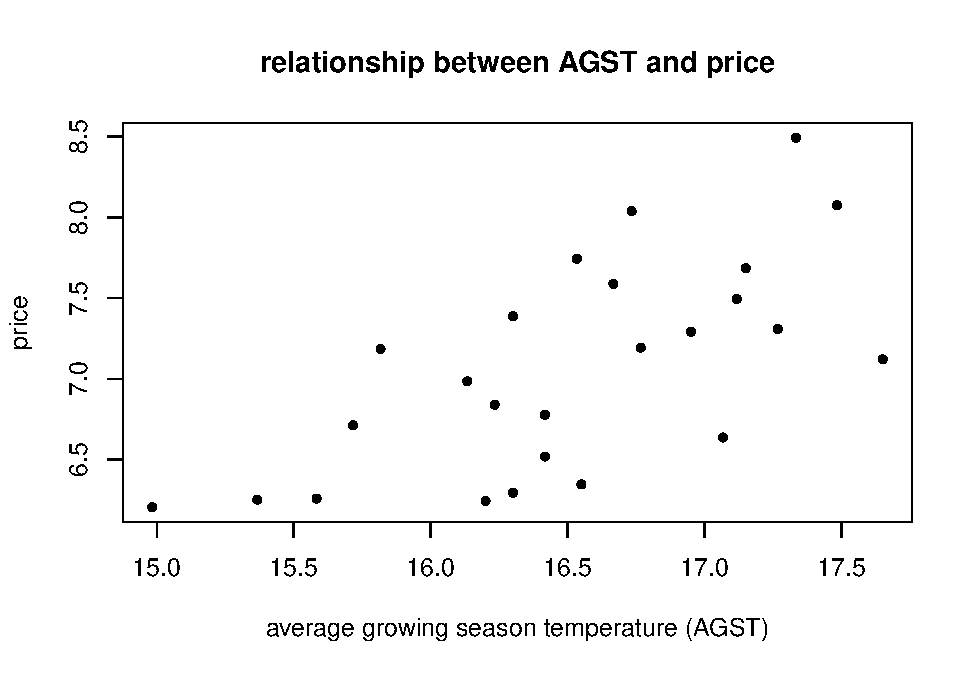
\includegraphics{HW2_Liu-Zi-Jian_files/figure-latex/unnamed-chunk-20-1.pdf}

\begin{Shaded}
\begin{Highlighting}[]
\KeywordTok{plot}\NormalTok{(wineData}\OperatorTok{$}\NormalTok{WinterRain, wineData}\OperatorTok{$}\NormalTok{Price, }\DataTypeTok{main=}\StringTok{"relationship between winterRain and price"}\NormalTok{,}
   \DataTypeTok{xlab=}\StringTok{"winter rain amount"}\NormalTok{, }\DataTypeTok{ylab=}\StringTok{"price"}\NormalTok{, }\DataTypeTok{pch=}\DecValTok{20}\NormalTok{)}
\end{Highlighting}
\end{Shaded}

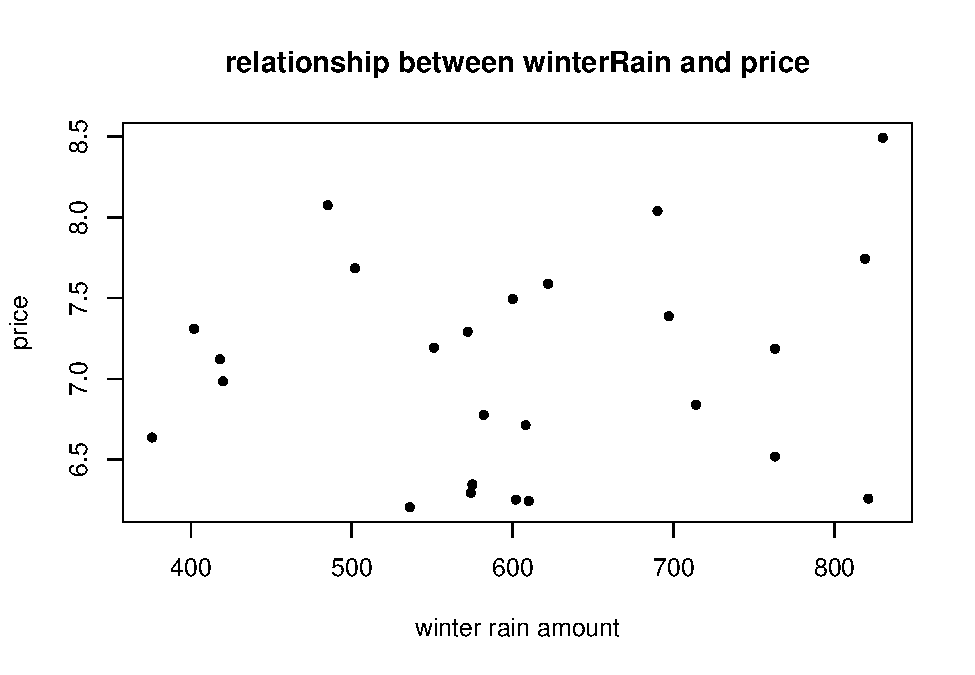
\includegraphics{HW2_Liu-Zi-Jian_files/figure-latex/unnamed-chunk-20-2.pdf}

\begin{Shaded}
\begin{Highlighting}[]
\KeywordTok{plot}\NormalTok{(wineData}\OperatorTok{$}\NormalTok{HarvestRain, wineData}\OperatorTok{$}\NormalTok{Price, }\DataTypeTok{main=}\StringTok{"relationship between harvest rain and price"}\NormalTok{,}
   \DataTypeTok{xlab=}\StringTok{"Harvest rain amount"}\NormalTok{, }\DataTypeTok{ylab=}\StringTok{"price"}\NormalTok{, }\DataTypeTok{pch=}\DecValTok{20}\NormalTok{)}
\end{Highlighting}
\end{Shaded}

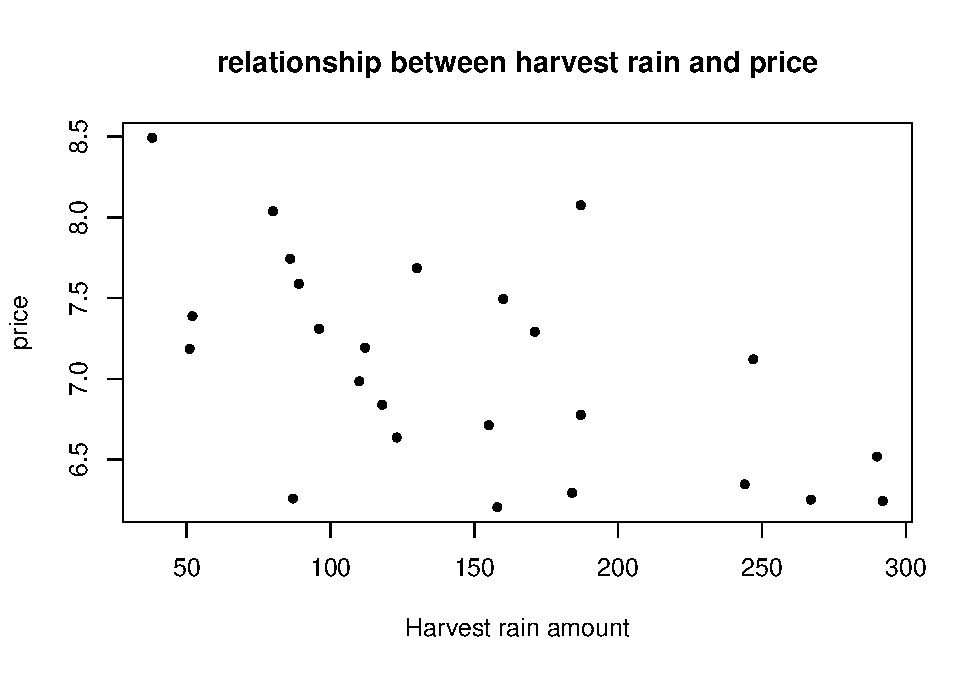
\includegraphics{HW2_Liu-Zi-Jian_files/figure-latex/unnamed-chunk-20-3.pdf}

\begin{Shaded}
\begin{Highlighting}[]
\KeywordTok{plot}\NormalTok{(wineData}\OperatorTok{$}\NormalTok{Age, wineData}\OperatorTok{$}\NormalTok{Price, }\DataTypeTok{main=}\StringTok{"relationship between age and price"}\NormalTok{,}
   \DataTypeTok{xlab=}\StringTok{"age of wine"}\NormalTok{, }\DataTypeTok{ylab=}\StringTok{"price"}\NormalTok{, }\DataTypeTok{pch=}\DecValTok{20}\NormalTok{)}
\end{Highlighting}
\end{Shaded}

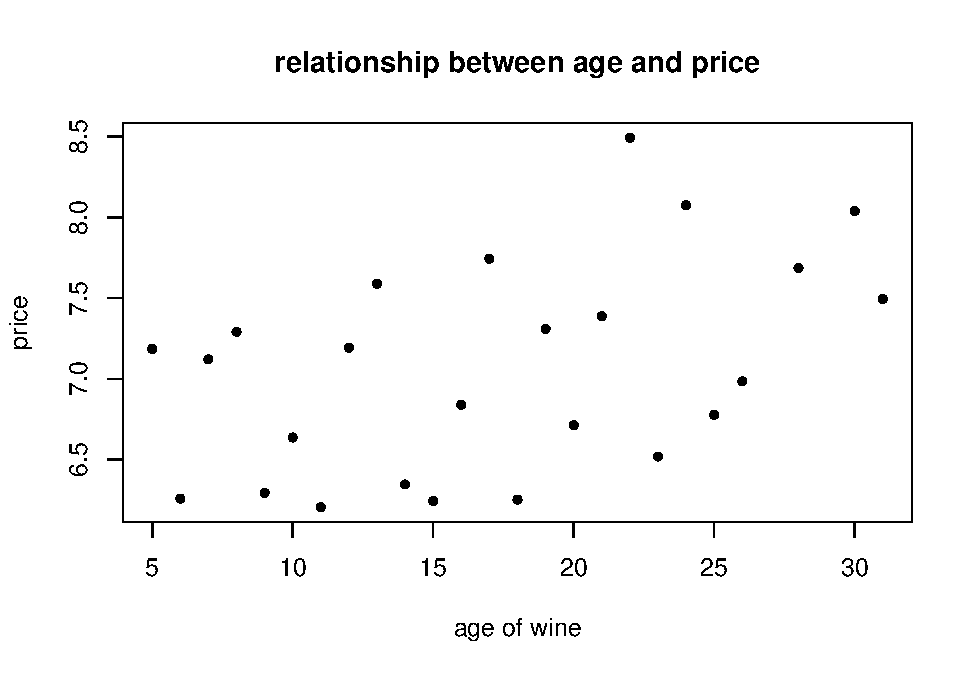
\includegraphics{HW2_Liu-Zi-Jian_files/figure-latex/unnamed-chunk-20-4.pdf}

The variable that looks to be the most correlated with Price would be
AGST. The scatter plot looks the most patterned and we see that
generally, the price increases as AGST increases, an upwards trend.

\begin{Shaded}
\begin{Highlighting}[]
\NormalTok{AGST <-}\StringTok{ }\KeywordTok{cor.test}\NormalTok{(wineData}\OperatorTok{$}\NormalTok{AGST, wineData}\OperatorTok{$}\NormalTok{Price, }
                    \DataTypeTok{method =} \StringTok{"pearson"}\NormalTok{)}
\NormalTok{winterRain <-}\StringTok{ }\KeywordTok{cor.test}\NormalTok{(wineData}\OperatorTok{$}\NormalTok{WinterRain, wineData}\OperatorTok{$}\NormalTok{Price, }
                    \DataTypeTok{method =} \StringTok{"pearson"}\NormalTok{)}
\NormalTok{harvestRain <-}\StringTok{ }\KeywordTok{cor.test}\NormalTok{(wineData}\OperatorTok{$}\NormalTok{HarvestRain, wineData}\OperatorTok{$}\NormalTok{Price, }
                    \DataTypeTok{method =} \StringTok{"pearson"}\NormalTok{)}
\NormalTok{ageWine <-}\StringTok{ }\KeywordTok{cor.test}\NormalTok{(wineData}\OperatorTok{$}\NormalTok{Age, wineData}\OperatorTok{$}\NormalTok{Price, }
                    \DataTypeTok{method =} \StringTok{"pearson"}\NormalTok{)}
\NormalTok{AGST}
\end{Highlighting}
\end{Shaded}

\begin{verbatim}
## 
##  Pearson's product-moment correlation
## 
## data:  wineData$AGST and wineData$Price
## t = 4.2083, df = 23, p-value = 0.000335
## alternative hypothesis: true correlation is not equal to 0
## 95 percent confidence interval:
##  0.3576371 0.8366511
## sample estimates:
##       cor 
## 0.6595629
\end{verbatim}

\begin{Shaded}
\begin{Highlighting}[]
\NormalTok{winterRain}
\end{Highlighting}
\end{Shaded}

\begin{verbatim}
## 
##  Pearson's product-moment correlation
## 
## data:  wineData$WinterRain and wineData$Price
## t = 0.66156, df = 23, p-value = 0.5148
## alternative hypothesis: true correlation is not equal to 0
## 95 percent confidence interval:
##  -0.2732336  0.5045389
## sample estimates:
##       cor 
## 0.1366505
\end{verbatim}

\begin{Shaded}
\begin{Highlighting}[]
\NormalTok{harvestRain}
\end{Highlighting}
\end{Shaded}

\begin{verbatim}
## 
##  Pearson's product-moment correlation
## 
## data:  wineData$HarvestRain and wineData$Price
## t = -3.2698, df = 23, p-value = 0.003366
## alternative hypothesis: true correlation is not equal to 0
## 95 percent confidence interval:
##  -0.7839554 -0.2163467
## sample estimates:
##        cor 
## -0.5633219
\end{verbatim}

\begin{Shaded}
\begin{Highlighting}[]
\NormalTok{ageWine}
\end{Highlighting}
\end{Shaded}

\begin{verbatim}
## 
##  Pearson's product-moment correlation
## 
## data:  wineData$Age and wineData$Price
## t = 2.4016, df = 23, p-value = 0.0248
## alternative hypothesis: true correlation is not equal to 0
## 95 percent confidence interval:
##  0.06395174 0.71618615
## sample estimates:
##       cor 
## 0.4477679
\end{verbatim}

As we can see from the pearson's correlation scores above, the cor of
0.6596 for AGST is the highest correlation between a variable and price.
This backs up our claim before that AGST is the most correlated with
price.

\hypertarget{part-ii.-marginal-regression-analysis}{%
\subsection{3. Part II. Marginal Regression
Analysis}\label{part-ii.-marginal-regression-analysis}}

\begin{Shaded}
\begin{Highlighting}[]
\CommentTok{# install.packages("rlang")}
\KeywordTok{library}\NormalTok{(rlang)}
\end{Highlighting}
\end{Shaded}

\begin{verbatim}
## Warning: package 'rlang' was built under R version 4.0.3
\end{verbatim}

\begin{Shaded}
\begin{Highlighting}[]
\CommentTok{#install.packages('ggplot2')}
\KeywordTok{library}\NormalTok{(ggplot2)}
\end{Highlighting}
\end{Shaded}

\begin{verbatim}
## Warning: package 'ggplot2' was built under R version 4.0.3
\end{verbatim}

\begin{Shaded}
\begin{Highlighting}[]
\CommentTok{#install.packages('sjPlot')}
\KeywordTok{library}\NormalTok{(sjPlot)}
\end{Highlighting}
\end{Shaded}

\begin{verbatim}
## Warning: package 'sjPlot' was built under R version 4.0.3
\end{verbatim}

\begin{verbatim}
## Learn more about sjPlot with 'browseVignettes("sjPlot")'.
\end{verbatim}

\begin{Shaded}
\begin{Highlighting}[]
\NormalTok{fit <-}\StringTok{ }\KeywordTok{lm}\NormalTok{(Price }\OperatorTok{~}\StringTok{ }\NormalTok{AGST, }\DataTypeTok{data =}\NormalTok{ wineData)}
\KeywordTok{plot_model}\NormalTok{(fit, }\DataTypeTok{type =} \StringTok{"pred"}\NormalTok{)}
\end{Highlighting}
\end{Shaded}

\begin{verbatim}
## $AGST
\end{verbatim}

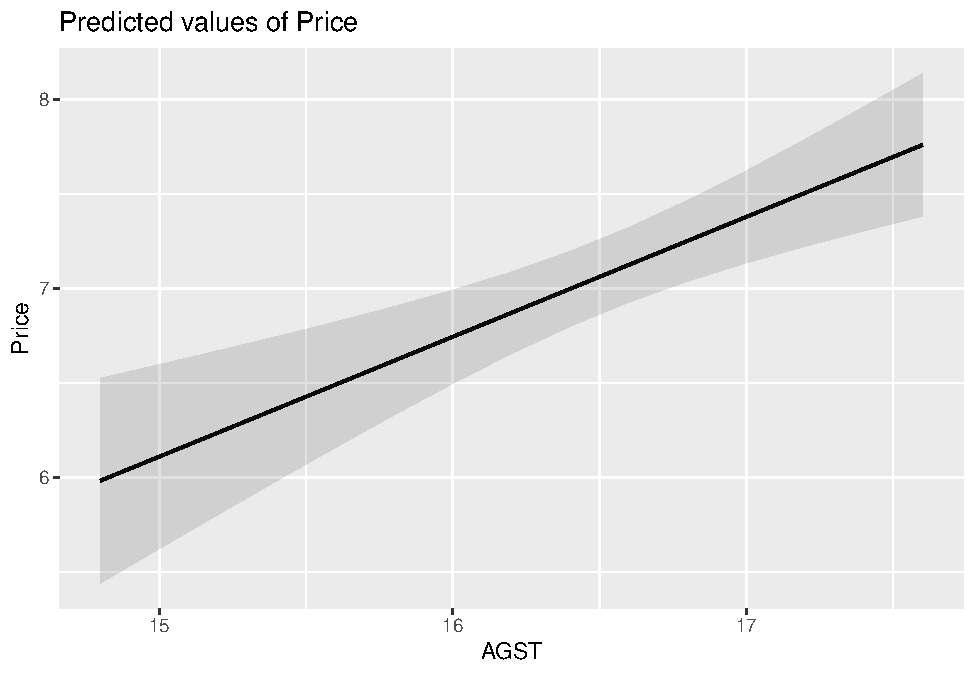
\includegraphics{HW2_Liu-Zi-Jian_files/figure-latex/unnamed-chunk-24-1.pdf}

\begin{Shaded}
\begin{Highlighting}[]
\KeywordTok{summary}\NormalTok{(fit)}
\end{Highlighting}
\end{Shaded}

\begin{verbatim}
## 
## Call:
## lm(formula = Price ~ AGST, data = wineData)
## 
## Residuals:
##      Min       1Q   Median       3Q      Max 
## -0.78450 -0.23882 -0.03727  0.38992  0.90318 
## 
## Coefficients:
##             Estimate Std. Error t value Pr(>|t|)    
## (Intercept)  -3.4178     2.4935  -1.371 0.183710    
## AGST          0.6351     0.1509   4.208 0.000335 ***
## ---
## Signif. codes:  0 '***' 0.001 '**' 0.01 '*' 0.05 '.' 0.1 ' ' 1
## 
## Residual standard error: 0.4993 on 23 degrees of freedom
## Multiple R-squared:  0.435,  Adjusted R-squared:  0.4105 
## F-statistic: 17.71 on 1 and 23 DF,  p-value: 0.000335
\end{verbatim}

The fitted coefficient values is -3.4178 and 0.6351. The intercept is
-3.4178 and the slope is 0.6351. For every 1 unit increase in AGST,
price increases by 0.6351. The Rsquared value is 0.435.

\hypertarget{part-iii.-multiple-regression-analysis}{%
\subsection{3. Part III. Multiple Regression
Analysis}\label{part-iii.-multiple-regression-analysis}}

\begin{Shaded}
\begin{Highlighting}[]
\NormalTok{multi_fit2 =}\StringTok{ }\KeywordTok{lm}\NormalTok{(Price }\OperatorTok{~}\StringTok{ }\NormalTok{AGST }\OperatorTok{+}\StringTok{ }\NormalTok{HarvestRain, }\DataTypeTok{data =}\NormalTok{ wineData)}
\KeywordTok{summary}\NormalTok{(multi_fit2)}
\end{Highlighting}
\end{Shaded}

\begin{verbatim}
## 
## Call:
## lm(formula = Price ~ AGST + HarvestRain, data = wineData)
## 
## Residuals:
##      Min       1Q   Median       3Q      Max 
## -0.88321 -0.19600  0.06178  0.15379  0.59722 
## 
## Coefficients:
##             Estimate Std. Error t value Pr(>|t|)    
## (Intercept) -2.20265    1.85443  -1.188 0.247585    
## AGST         0.60262    0.11128   5.415 1.94e-05 ***
## HarvestRain -0.00457    0.00101  -4.525 0.000167 ***
## ---
## Signif. codes:  0 '***' 0.001 '**' 0.01 '*' 0.05 '.' 0.1 ' ' 1
## 
## Residual standard error: 0.3674 on 22 degrees of freedom
## Multiple R-squared:  0.7074, Adjusted R-squared:  0.6808 
## F-statistic: 26.59 on 2 and 22 DF,  p-value: 1.347e-06
\end{verbatim}

\begin{Shaded}
\begin{Highlighting}[]
\NormalTok{multi_fit3 =}\StringTok{ }\KeywordTok{lm}\NormalTok{(Price }\OperatorTok{~}\StringTok{ }\NormalTok{AGST }\OperatorTok{+}\StringTok{ }\NormalTok{HarvestRain }\OperatorTok{+}\StringTok{ }\NormalTok{Age, }\DataTypeTok{data =}\NormalTok{ wineData)}
\KeywordTok{summary}\NormalTok{(multi_fit3)}
\end{Highlighting}
\end{Shaded}

\begin{verbatim}
## 
## Call:
## lm(formula = Price ~ AGST + HarvestRain + Age, data = wineData)
## 
## Residuals:
##      Min       1Q   Median       3Q      Max 
## -0.66258 -0.22953 -0.00268  0.27236  0.49391 
## 
## Coefficients:
##               Estimate Std. Error t value Pr(>|t|)    
## (Intercept) -1.4778196  1.6274142  -0.908  0.37414    
## AGST         0.5322922  0.0995343   5.348 2.65e-05 ***
## HarvestRain -0.0045386  0.0008757  -5.183 3.90e-05 ***
## Age          0.0250875  0.0087249   2.875  0.00905 ** 
## ---
## Signif. codes:  0 '***' 0.001 '**' 0.01 '*' 0.05 '.' 0.1 ' ' 1
## 
## Residual standard error: 0.3186 on 21 degrees of freedom
## Multiple R-squared:   0.79,  Adjusted R-squared:   0.76 
## F-statistic: 26.34 on 3 and 21 DF,  p-value: 2.596e-07
\end{verbatim}

\begin{Shaded}
\begin{Highlighting}[]
\NormalTok{multi_fit4 =}\StringTok{ }\KeywordTok{lm}\NormalTok{(Price }\OperatorTok{~}\StringTok{ }\NormalTok{AGST }\OperatorTok{+}\StringTok{ }\NormalTok{HarvestRain }\OperatorTok{+}\StringTok{ }\NormalTok{Age }\OperatorTok{+}\StringTok{ }\NormalTok{WinterRain, }\DataTypeTok{data =}\NormalTok{ wineData)}
\KeywordTok{summary}\NormalTok{(multi_fit4)}
\end{Highlighting}
\end{Shaded}

\begin{verbatim}
## 
## Call:
## lm(formula = Price ~ AGST + HarvestRain + Age + WinterRain, data = wineData)
## 
## Residuals:
##      Min       1Q   Median       3Q      Max 
## -0.45470 -0.24273  0.00752  0.19773  0.53637 
## 
## Coefficients:
##               Estimate Std. Error t value Pr(>|t|)    
## (Intercept) -3.4299802  1.7658975  -1.942 0.066311 .  
## AGST         0.6072093  0.0987022   6.152  5.2e-06 ***
## HarvestRain -0.0039715  0.0008538  -4.652 0.000154 ***
## Age          0.0239308  0.0080969   2.956 0.007819 ** 
## WinterRain   0.0010755  0.0005073   2.120 0.046694 *  
## ---
## Signif. codes:  0 '***' 0.001 '**' 0.01 '*' 0.05 '.' 0.1 ' ' 1
## 
## Residual standard error: 0.295 on 20 degrees of freedom
## Multiple R-squared:  0.8286, Adjusted R-squared:  0.7943 
## F-statistic: 24.17 on 4 and 20 DF,  p-value: 2.036e-07
\end{verbatim}

\begin{Shaded}
\begin{Highlighting}[]
\NormalTok{multi_fit5 =}\StringTok{ }\KeywordTok{lm}\NormalTok{(Price }\OperatorTok{~}\StringTok{ }\NormalTok{AGST }\OperatorTok{+}\StringTok{ }\NormalTok{HarvestRain }\OperatorTok{+}\StringTok{ }\NormalTok{Age }\OperatorTok{+}\StringTok{ }\NormalTok{WinterRain }\OperatorTok{+}\StringTok{ }\NormalTok{FrancePop, }\DataTypeTok{data =}\NormalTok{ wineData)}
\KeywordTok{summary}\NormalTok{(multi_fit5)}
\end{Highlighting}
\end{Shaded}

\begin{verbatim}
## 
## Call:
## lm(formula = Price ~ AGST + HarvestRain + Age + WinterRain + 
##     FrancePop, data = wineData)
## 
## Residuals:
##      Min       1Q   Median       3Q      Max 
## -0.48179 -0.24662 -0.00726  0.22012  0.51987 
## 
## Coefficients:
##               Estimate Std. Error t value Pr(>|t|)    
## (Intercept) -4.504e-01  1.019e+01  -0.044 0.965202    
## AGST         6.012e-01  1.030e-01   5.836 1.27e-05 ***
## HarvestRain -3.958e-03  8.751e-04  -4.523 0.000233 ***
## Age          5.847e-04  7.900e-02   0.007 0.994172    
## WinterRain   1.043e-03  5.310e-04   1.963 0.064416 .  
## FrancePop   -4.953e-05  1.667e-04  -0.297 0.769578    
## ---
## Signif. codes:  0 '***' 0.001 '**' 0.01 '*' 0.05 '.' 0.1 ' ' 1
## 
## Residual standard error: 0.3019 on 19 degrees of freedom
## Multiple R-squared:  0.8294, Adjusted R-squared:  0.7845 
## F-statistic: 18.47 on 5 and 19 DF,  p-value: 1.044e-06
\end{verbatim}

As we add more covriates, we find that R squared on the training data
increases. Which generally could mean that the model is fitted better.
We find that at 1 variable, Rsquared = 0.435, increasing to 0.7074,
0.79, 0.8286, and finally 0.8294 at 5 covariates. The model that we
choose based on Rsquared is Price \textasciitilde{} AGST + HarvestRain +
Age + WinterRain + FrancePop since the Rsquared is the highest. Note:
sometimes having a high Rsquared does not lead to a better model.

\begin{Shaded}
\begin{Highlighting}[]
\NormalTok{winetestData <-}\StringTok{ }\KeywordTok{read.csv}\NormalTok{(}\StringTok{'_data_hw2/winetest.csv'}\NormalTok{)}
\KeywordTok{head}\NormalTok{(winetestData)}
\end{Highlighting}
\end{Shaded}

\begin{verbatim}
##   Year  Price WinterRain    AGST HarvestRain Age FrancePop
## 1 1979 6.9541        717 16.1667         122   4  54835.83
## 2 1980 6.4979        578 16.0000          74   3  55110.24
\end{verbatim}

\begin{Shaded}
\begin{Highlighting}[]
\NormalTok{testfit <-}\StringTok{ }\KeywordTok{lm}\NormalTok{(Price }\OperatorTok{~}\StringTok{ }\NormalTok{AGST, }\DataTypeTok{data =}\NormalTok{ winetestData)}
\KeywordTok{summary}\NormalTok{(testfit)}
\end{Highlighting}
\end{Shaded}

\begin{verbatim}
## 
## Call:
## lm(formula = Price ~ AGST, data = winetestData)
## 
## Residuals:
## ALL 2 residuals are 0: no residual degrees of freedom!
## 
## Coefficients:
##             Estimate Std. Error t value Pr(>|t|)
## (Intercept)  -37.289         NA      NA       NA
## AGST           2.737         NA      NA       NA
## 
## Residual standard error: NaN on 0 degrees of freedom
## Multiple R-squared:      1,  Adjusted R-squared:    NaN 
## F-statistic:   NaN on 1 and 0 DF,  p-value: NA
\end{verbatim}

\begin{Shaded}
\begin{Highlighting}[]
\NormalTok{testmulti_fit2 =}\StringTok{ }\KeywordTok{lm}\NormalTok{(Price }\OperatorTok{~}\StringTok{ }\NormalTok{AGST }\OperatorTok{+}\StringTok{ }\NormalTok{HarvestRain, }\DataTypeTok{data =}\NormalTok{ winetestData)}
\KeywordTok{summary}\NormalTok{(testmulti_fit2)}
\end{Highlighting}
\end{Shaded}

\begin{verbatim}
## 
## Call:
## lm(formula = Price ~ AGST + HarvestRain, data = winetestData)
## 
## Residuals:
## ALL 2 residuals are 0: no residual degrees of freedom!
## 
## Coefficients: (1 not defined because of singularities)
##             Estimate Std. Error t value Pr(>|t|)
## (Intercept)  -37.289         NA      NA       NA
## AGST           2.737         NA      NA       NA
## HarvestRain       NA         NA      NA       NA
## 
## Residual standard error: NaN on 0 degrees of freedom
## Multiple R-squared:      1,  Adjusted R-squared:    NaN 
## F-statistic:   NaN on 1 and 0 DF,  p-value: NA
\end{verbatim}

\begin{Shaded}
\begin{Highlighting}[]
\NormalTok{testmulti_fit3 =}\StringTok{ }\KeywordTok{lm}\NormalTok{(Price }\OperatorTok{~}\StringTok{ }\NormalTok{AGST }\OperatorTok{+}\StringTok{ }\NormalTok{HarvestRain }\OperatorTok{+}\StringTok{ }\NormalTok{Age, }\DataTypeTok{data =}\NormalTok{ winetestData)}
\KeywordTok{summary}\NormalTok{(testmulti_fit3)}
\end{Highlighting}
\end{Shaded}

\begin{verbatim}
## 
## Call:
## lm(formula = Price ~ AGST + HarvestRain + Age, data = winetestData)
## 
## Residuals:
## ALL 2 residuals are 0: no residual degrees of freedom!
## 
## Coefficients: (2 not defined because of singularities)
##             Estimate Std. Error t value Pr(>|t|)
## (Intercept)  -37.289         NA      NA       NA
## AGST           2.737         NA      NA       NA
## HarvestRain       NA         NA      NA       NA
## Age               NA         NA      NA       NA
## 
## Residual standard error: NaN on 0 degrees of freedom
## Multiple R-squared:      1,  Adjusted R-squared:    NaN 
## F-statistic:   NaN on 1 and 0 DF,  p-value: NA
\end{verbatim}

\begin{Shaded}
\begin{Highlighting}[]
\NormalTok{testmulti_fit4 =}\StringTok{ }\KeywordTok{lm}\NormalTok{(Price }\OperatorTok{~}\StringTok{ }\NormalTok{AGST }\OperatorTok{+}\StringTok{ }\NormalTok{HarvestRain }\OperatorTok{+}\StringTok{ }\NormalTok{Age }\OperatorTok{+}\StringTok{ }\NormalTok{WinterRain, }\DataTypeTok{data =}\NormalTok{ winetestData)}
\KeywordTok{summary}\NormalTok{(testmulti_fit4)}
\end{Highlighting}
\end{Shaded}

\begin{verbatim}
## 
## Call:
## lm(formula = Price ~ AGST + HarvestRain + Age + WinterRain, data = winetestData)
## 
## Residuals:
## ALL 2 residuals are 0: no residual degrees of freedom!
## 
## Coefficients: (3 not defined because of singularities)
##             Estimate Std. Error t value Pr(>|t|)
## (Intercept)  -37.289         NA      NA       NA
## AGST           2.737         NA      NA       NA
## HarvestRain       NA         NA      NA       NA
## Age               NA         NA      NA       NA
## WinterRain        NA         NA      NA       NA
## 
## Residual standard error: NaN on 0 degrees of freedom
## Multiple R-squared:      1,  Adjusted R-squared:    NaN 
## F-statistic:   NaN on 1 and 0 DF,  p-value: NA
\end{verbatim}

\begin{Shaded}
\begin{Highlighting}[]
\NormalTok{testmulti_fit5 =}\StringTok{ }\KeywordTok{lm}\NormalTok{(Price }\OperatorTok{~}\StringTok{ }\NormalTok{AGST }\OperatorTok{+}\StringTok{ }\NormalTok{HarvestRain }\OperatorTok{+}\StringTok{ }\NormalTok{Age }\OperatorTok{+}\StringTok{ }\NormalTok{WinterRain }\OperatorTok{+}\StringTok{ }\NormalTok{FrancePop, }\DataTypeTok{data =}\NormalTok{ winetestData)}
\KeywordTok{summary}\NormalTok{(testmulti_fit5)}
\end{Highlighting}
\end{Shaded}

\begin{verbatim}
## 
## Call:
## lm(formula = Price ~ AGST + HarvestRain + Age + WinterRain + 
##     FrancePop, data = winetestData)
## 
## Residuals:
## ALL 2 residuals are 0: no residual degrees of freedom!
## 
## Coefficients: (4 not defined because of singularities)
##             Estimate Std. Error t value Pr(>|t|)
## (Intercept)  -37.289         NA      NA       NA
## AGST           2.737         NA      NA       NA
## HarvestRain       NA         NA      NA       NA
## Age               NA         NA      NA       NA
## WinterRain        NA         NA      NA       NA
## FrancePop         NA         NA      NA       NA
## 
## Residual standard error: NaN on 0 degrees of freedom
## Multiple R-squared:      1,  Adjusted R-squared:    NaN 
## F-statistic:   NaN on 1 and 0 DF,  p-value: NA
\end{verbatim}

From the winetest data provided, since all of the variables is collinear
to AGST, adding covariates does not change the Rsquared and the
coefficient values. Also there is only 2 data entries. The Rsquared
value for each model is equal to 1. The model that we choose based on
Rsquared is Price \textasciitilde{} AGST since all of the variables are
collinear.

\begin{Shaded}
\begin{Highlighting}[]
\NormalTok{multi_fit5 =}\StringTok{ }\KeywordTok{lm}\NormalTok{(Price }\OperatorTok{~}\StringTok{ }\NormalTok{AGST }\OperatorTok{+}\StringTok{ }\NormalTok{HarvestRain }\OperatorTok{+}\StringTok{ }\NormalTok{Age }\OperatorTok{+}\StringTok{ }\NormalTok{WinterRain }\OperatorTok{+}\StringTok{ }\NormalTok{FrancePop, }\DataTypeTok{data =}\NormalTok{ wineData)}
\KeywordTok{summary}\NormalTok{(multi_fit5)}
\end{Highlighting}
\end{Shaded}

\begin{verbatim}
## 
## Call:
## lm(formula = Price ~ AGST + HarvestRain + Age + WinterRain + 
##     FrancePop, data = wineData)
## 
## Residuals:
##      Min       1Q   Median       3Q      Max 
## -0.48179 -0.24662 -0.00726  0.22012  0.51987 
## 
## Coefficients:
##               Estimate Std. Error t value Pr(>|t|)    
## (Intercept) -4.504e-01  1.019e+01  -0.044 0.965202    
## AGST         6.012e-01  1.030e-01   5.836 1.27e-05 ***
## HarvestRain -3.958e-03  8.751e-04  -4.523 0.000233 ***
## Age          5.847e-04  7.900e-02   0.007 0.994172    
## WinterRain   1.043e-03  5.310e-04   1.963 0.064416 .  
## FrancePop   -4.953e-05  1.667e-04  -0.297 0.769578    
## ---
## Signif. codes:  0 '***' 0.001 '**' 0.01 '*' 0.05 '.' 0.1 ' ' 1
## 
## Residual standard error: 0.3019 on 19 degrees of freedom
## Multiple R-squared:  0.8294, Adjusted R-squared:  0.7845 
## F-statistic: 18.47 on 5 and 19 DF,  p-value: 1.044e-06
\end{verbatim}

As seen above, we can see that rains in the winter followed by hot
summer (high AGST) both has a positive relation with price. However the
hot summer affects the price of the wine a lot more than the rain in the
winter. Rainfall at harvest also has a negative relation with price. If
we take that the price reflects the quality of wine, then
Prof.~Ashenfelter's findings is consistent with our model.

\hypertarget{question-4.-moneyball}{%
\section{Question 4. Moneyball}\label{question-4.-moneyball}}

\hypertarget{part-i.-preliminary-analysis-1}{%
\section{4. Part I. Preliminary
Analysis}\label{part-i.-preliminary-analysis-1}}

\begin{Shaded}
\begin{Highlighting}[]
\NormalTok{baseballData <-}\StringTok{ }\KeywordTok{read.csv}\NormalTok{(}\StringTok{'_data_hw2/baseball.csv'}\NormalTok{)}
\KeywordTok{head}\NormalTok{(baseballData)}
\end{Highlighting}
\end{Shaded}

\begin{verbatim}
##   Team League Year  RS  RA  W   OBP   SLG    BA Playoffs RankSeason
## 1  ARI     NL 2012 734 688 81 0.328 0.418 0.259        0         NA
## 2  ATL     NL 2012 700 600 94 0.320 0.389 0.247        1          4
## 3  BAL     AL 2012 712 705 93 0.311 0.417 0.247        1          5
## 4  BOS     AL 2012 734 806 69 0.315 0.415 0.260        0         NA
## 5  CHC     NL 2012 613 759 61 0.302 0.378 0.240        0         NA
## 6  CHW     AL 2012 748 676 85 0.318 0.422 0.255        0         NA
##   RankPlayoffs   G  OOBP  OSLG
## 1           NA 162 0.317 0.415
## 2            5 162 0.306 0.378
## 3            4 162 0.315 0.403
## 4           NA 162 0.331 0.428
## 5           NA 162 0.335 0.424
## 6           NA 162 0.319 0.405
\end{verbatim}

\begin{Shaded}
\begin{Highlighting}[]
\KeywordTok{hist}\NormalTok{(baseballData}\OperatorTok{$}\NormalTok{OBP)}
\end{Highlighting}
\end{Shaded}

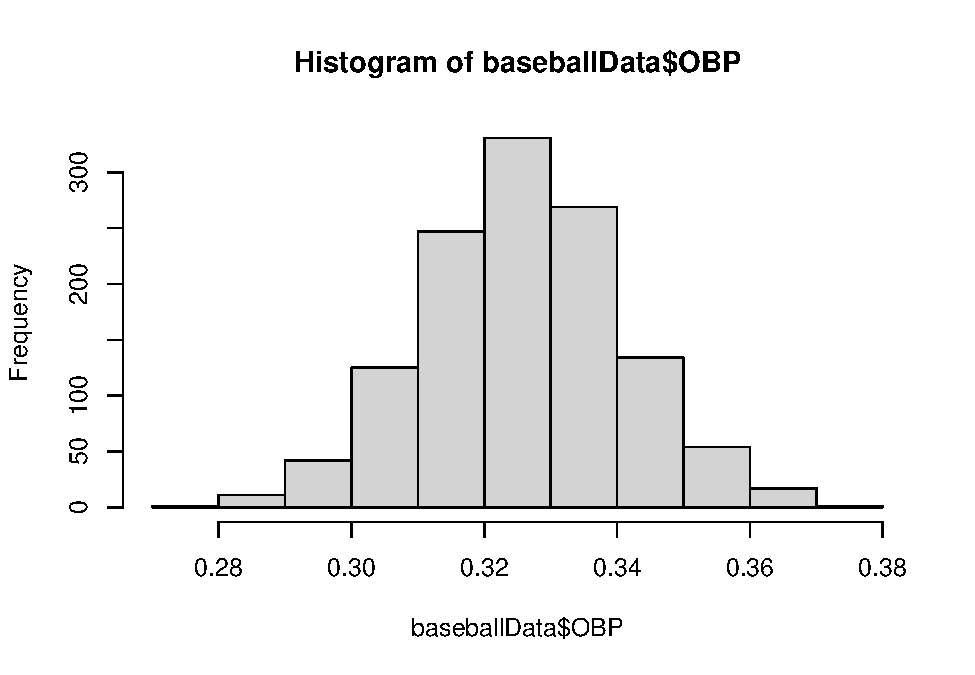
\includegraphics{HW2_Liu-Zi-Jian_files/figure-latex/unnamed-chunk-30-1.pdf}

\begin{Shaded}
\begin{Highlighting}[]
\KeywordTok{boxplot}\NormalTok{(baseballData}\OperatorTok{$}\NormalTok{OBP)}
\end{Highlighting}
\end{Shaded}

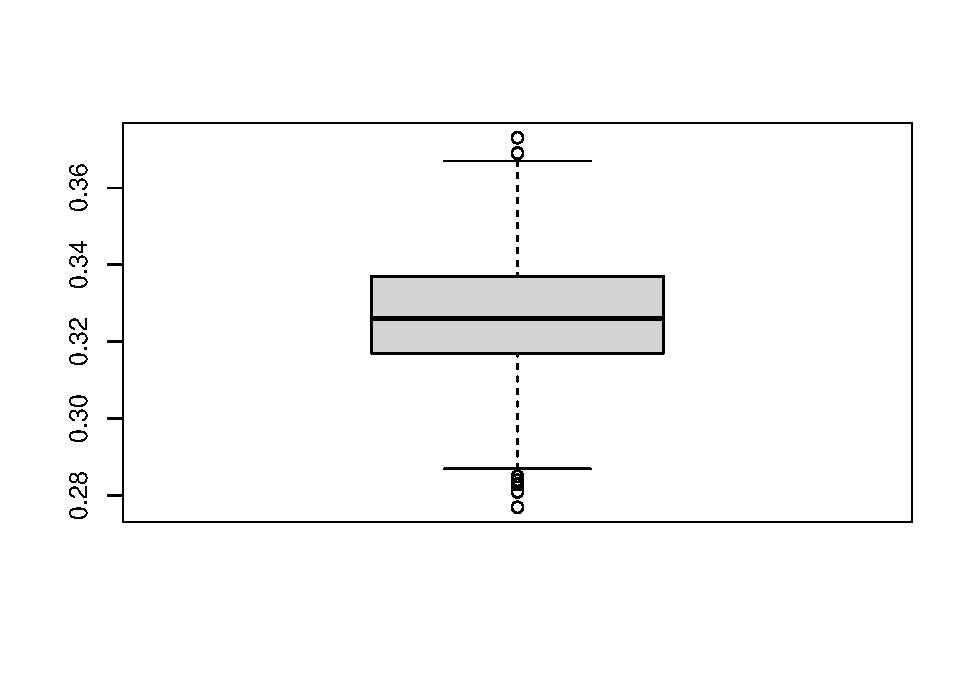
\includegraphics{HW2_Liu-Zi-Jian_files/figure-latex/unnamed-chunk-30-2.pdf}

\begin{Shaded}
\begin{Highlighting}[]
\KeywordTok{mean}\NormalTok{(baseballData}\OperatorTok{$}\NormalTok{OBP)}
\end{Highlighting}
\end{Shaded}

\begin{verbatim}
## [1] 0.3263312
\end{verbatim}

\begin{Shaded}
\begin{Highlighting}[]
\KeywordTok{median}\NormalTok{(baseballData}\OperatorTok{$}\NormalTok{OBP)}
\end{Highlighting}
\end{Shaded}

\begin{verbatim}
## [1] 0.326
\end{verbatim}

Histogram and boxplot for OBP. The mean and median of OBP is 0.3263312
and 0.326 respectively. This means that the distribution is not skewed.
You can also verify this from the boxplot and histogram.

\begin{Shaded}
\begin{Highlighting}[]
\KeywordTok{hist}\NormalTok{(baseballData}\OperatorTok{$}\NormalTok{SLG)}
\end{Highlighting}
\end{Shaded}

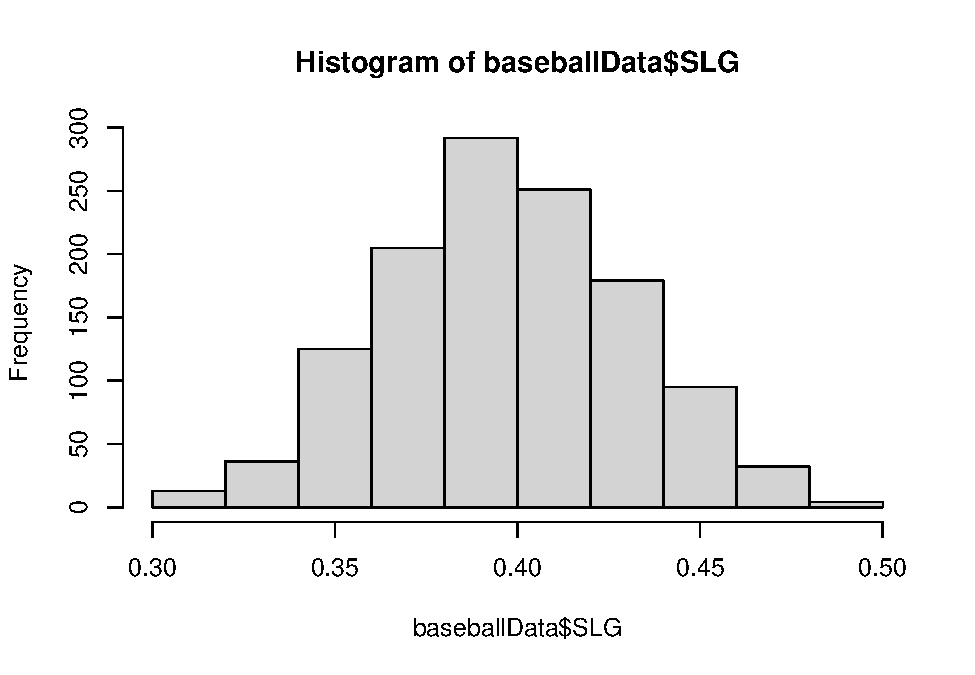
\includegraphics{HW2_Liu-Zi-Jian_files/figure-latex/unnamed-chunk-31-1.pdf}

\begin{Shaded}
\begin{Highlighting}[]
\KeywordTok{boxplot}\NormalTok{(baseballData}\OperatorTok{$}\NormalTok{SLG)}
\end{Highlighting}
\end{Shaded}

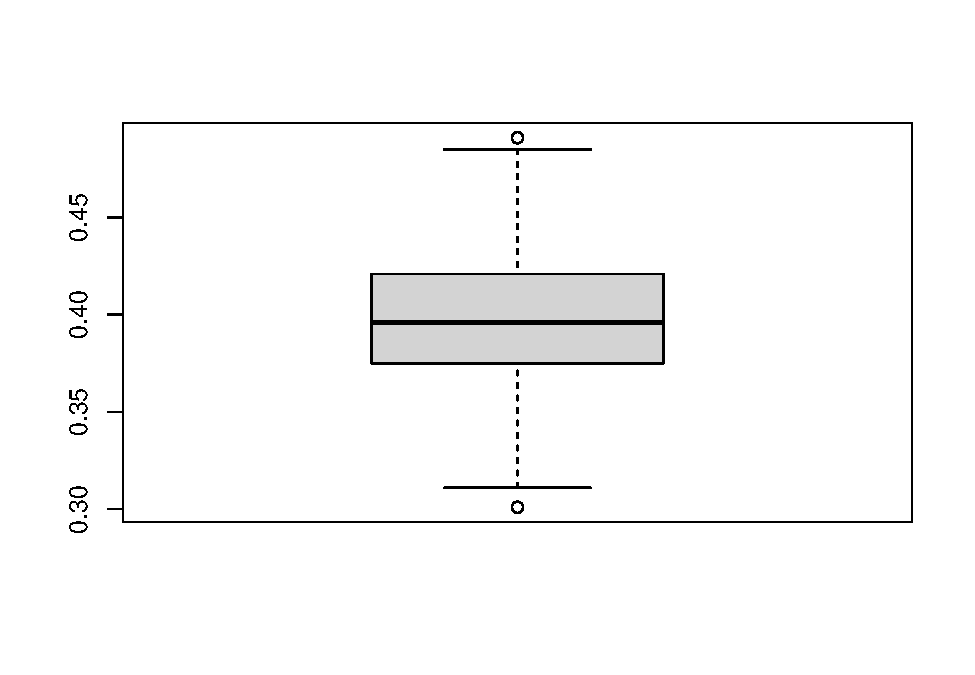
\includegraphics{HW2_Liu-Zi-Jian_files/figure-latex/unnamed-chunk-31-2.pdf}

\begin{Shaded}
\begin{Highlighting}[]
\KeywordTok{mean}\NormalTok{(baseballData}\OperatorTok{$}\NormalTok{SLG)}
\end{Highlighting}
\end{Shaded}

\begin{verbatim}
## [1] 0.3973417
\end{verbatim}

\begin{Shaded}
\begin{Highlighting}[]
\KeywordTok{median}\NormalTok{(baseballData}\OperatorTok{$}\NormalTok{SLG)}
\end{Highlighting}
\end{Shaded}

\begin{verbatim}
## [1] 0.396
\end{verbatim}

Histogram and boxplot for SLG. The mean and median of OBP is 0.3973417
and 0.396 respectively. This means that the distribution is not skewed.
You can also verify this from the boxplot and histogram.

\begin{Shaded}
\begin{Highlighting}[]
\KeywordTok{hist}\NormalTok{(baseballData}\OperatorTok{$}\NormalTok{BA)}
\end{Highlighting}
\end{Shaded}

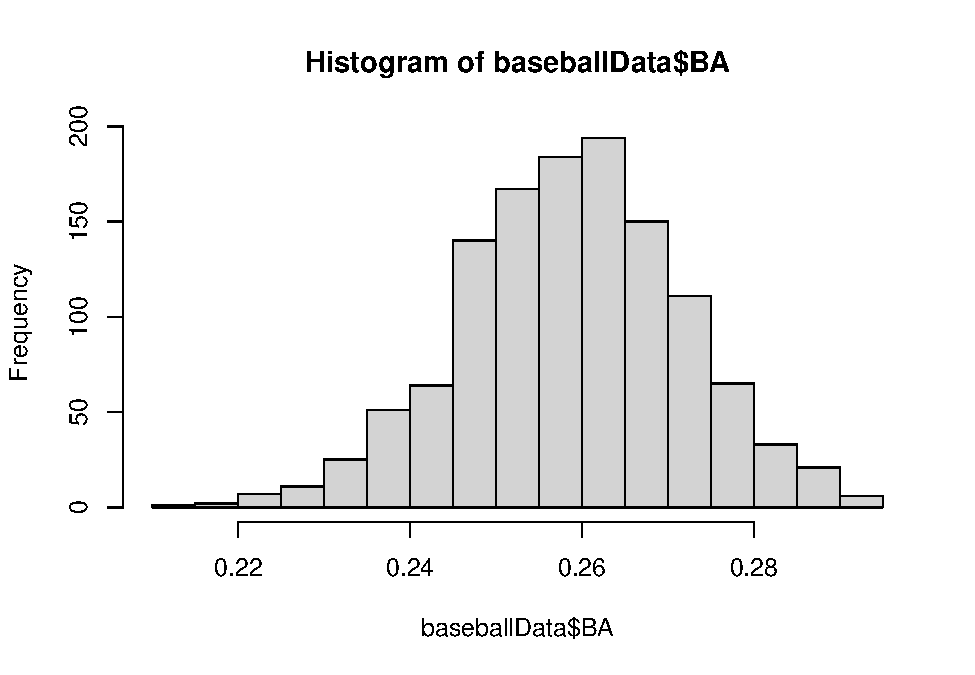
\includegraphics{HW2_Liu-Zi-Jian_files/figure-latex/unnamed-chunk-32-1.pdf}

\begin{Shaded}
\begin{Highlighting}[]
\KeywordTok{boxplot}\NormalTok{(baseballData}\OperatorTok{$}\NormalTok{BA)}
\end{Highlighting}
\end{Shaded}

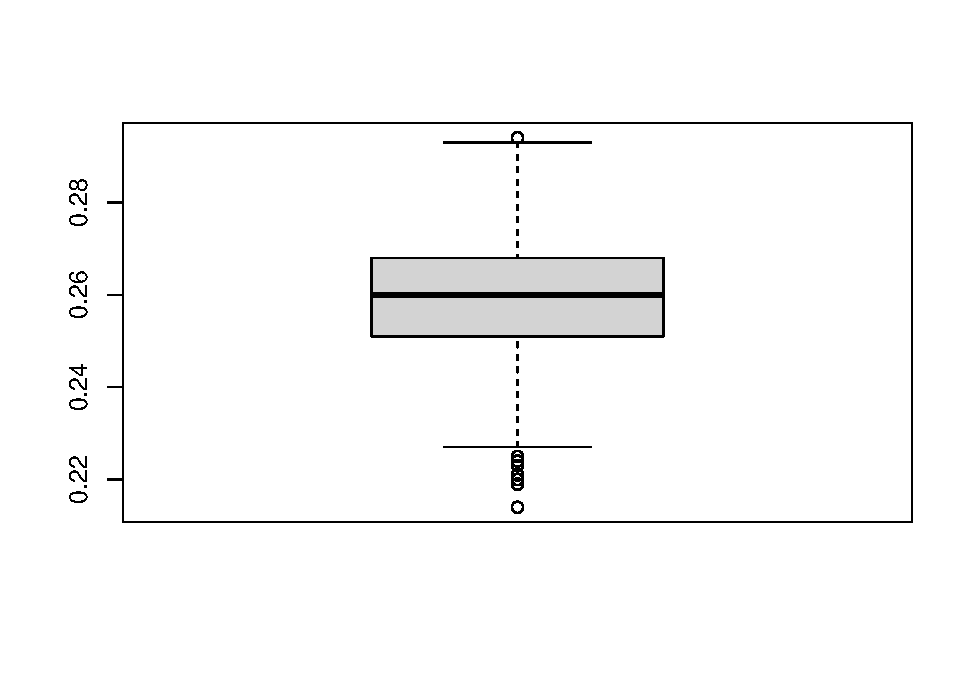
\includegraphics{HW2_Liu-Zi-Jian_files/figure-latex/unnamed-chunk-32-2.pdf}

\begin{Shaded}
\begin{Highlighting}[]
\KeywordTok{mean}\NormalTok{(baseballData}\OperatorTok{$}\NormalTok{BA)}
\end{Highlighting}
\end{Shaded}

\begin{verbatim}
## [1] 0.2592727
\end{verbatim}

\begin{Shaded}
\begin{Highlighting}[]
\KeywordTok{median}\NormalTok{(baseballData}\OperatorTok{$}\NormalTok{BA)}
\end{Highlighting}
\end{Shaded}

\begin{verbatim}
## [1] 0.26
\end{verbatim}

Histogram and boxplot for BA. The mean and median of OBP is 0.2592727
and 0.26 respectively. This means that the distribution is not skewed.
You can also verify this from the boxplot and histogram.

\hypertarget{part-ii.-marginal-regression-analysis-1}{%
\subsection{4. Part II. Marginal Regression
Analysis}\label{part-ii.-marginal-regression-analysis-1}}

\begin{Shaded}
\begin{Highlighting}[]
\NormalTok{BAfit <-}\StringTok{ }\KeywordTok{lm}\NormalTok{(RS }\OperatorTok{~}\StringTok{ }\NormalTok{BA, }\DataTypeTok{data =}\NormalTok{ baseballData)}
\KeywordTok{summary}\NormalTok{(BAfit)}
\end{Highlighting}
\end{Shaded}

\begin{verbatim}
## 
## Call:
## lm(formula = RS ~ BA, data = baseballData)
## 
## Residuals:
##      Min       1Q   Median       3Q      Max 
## -158.429  -36.057   -1.064   35.018  179.518 
## 
## Coefficients:
##             Estimate Std. Error t value Pr(>|t|)    
## (Intercept)  -805.51      29.51  -27.30   <2e-16 ***
## BA           5864.84     113.68   51.59   <2e-16 ***
## ---
## Signif. codes:  0 '***' 0.001 '**' 0.01 '*' 0.05 '.' 0.1 ' ' 1
## 
## Residual standard error: 51.48 on 1230 degrees of freedom
## Multiple R-squared:  0.6839, Adjusted R-squared:  0.6837 
## F-statistic:  2662 on 1 and 1230 DF,  p-value: < 2.2e-16
\end{verbatim}

\begin{Shaded}
\begin{Highlighting}[]
\KeywordTok{plot}\NormalTok{(baseballData}\OperatorTok{$}\NormalTok{BA, baseballData}\OperatorTok{$}\NormalTok{RS)}
\KeywordTok{abline}\NormalTok{(BAfit)}
\end{Highlighting}
\end{Shaded}

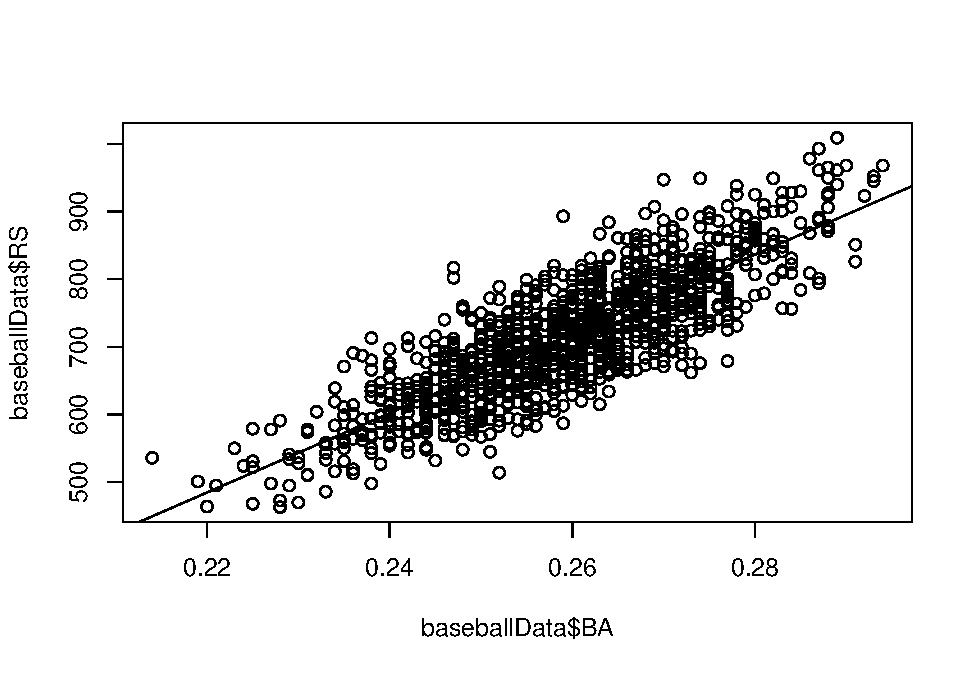
\includegraphics{HW2_Liu-Zi-Jian_files/figure-latex/unnamed-chunk-33-1.pdf}

Above is the scatter plot using model RS \textasciitilde{} BA. The
intercept and slope are -805.51, and 5864.84 respectively, the Rsquared
is 0.6839

\begin{Shaded}
\begin{Highlighting}[]
\KeywordTok{plot}\NormalTok{(BAfit)}
\end{Highlighting}
\end{Shaded}

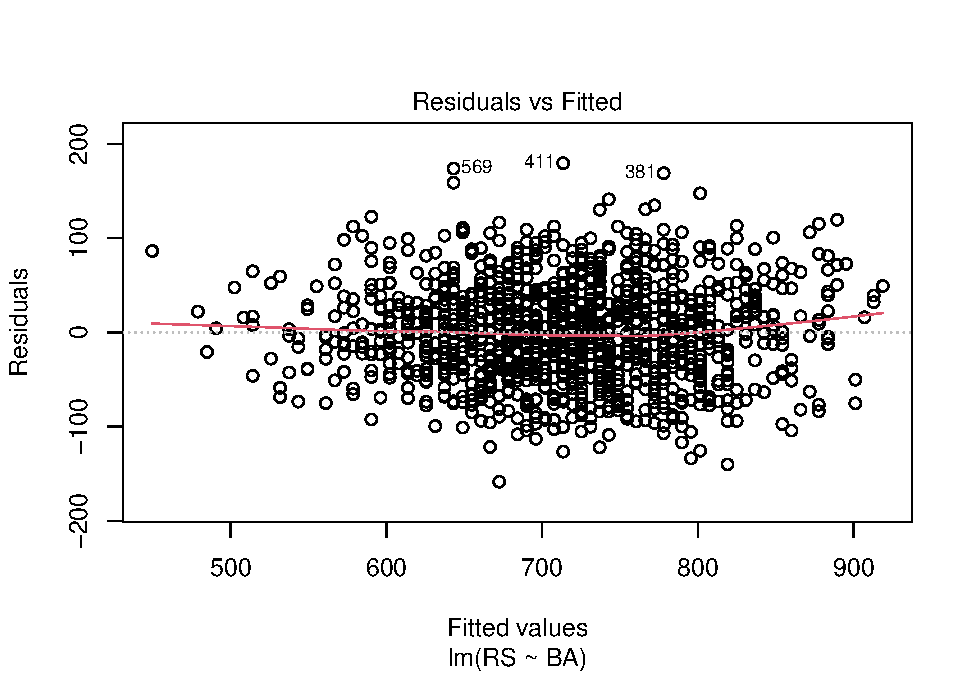
\includegraphics{HW2_Liu-Zi-Jian_files/figure-latex/unnamed-chunk-34-1.pdf}
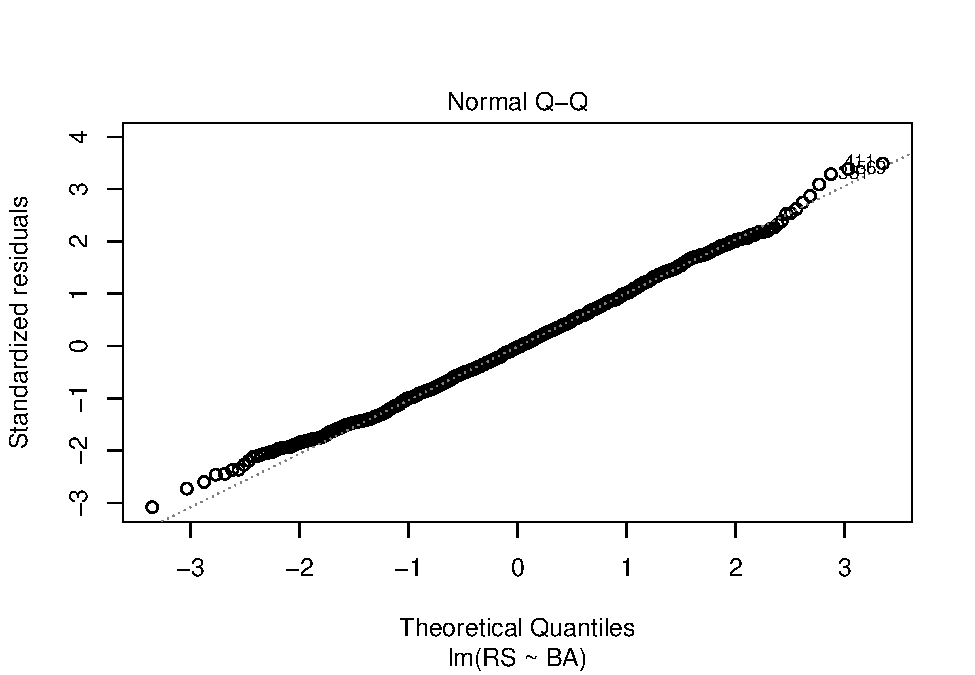
\includegraphics{HW2_Liu-Zi-Jian_files/figure-latex/unnamed-chunk-34-2.pdf}
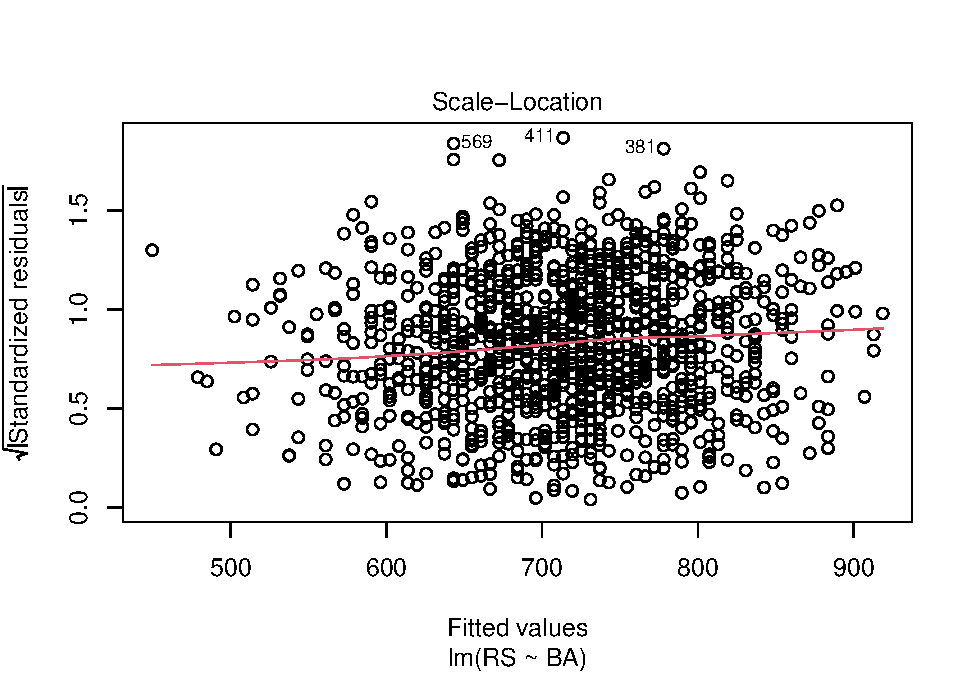
\includegraphics{HW2_Liu-Zi-Jian_files/figure-latex/unnamed-chunk-34-3.pdf}
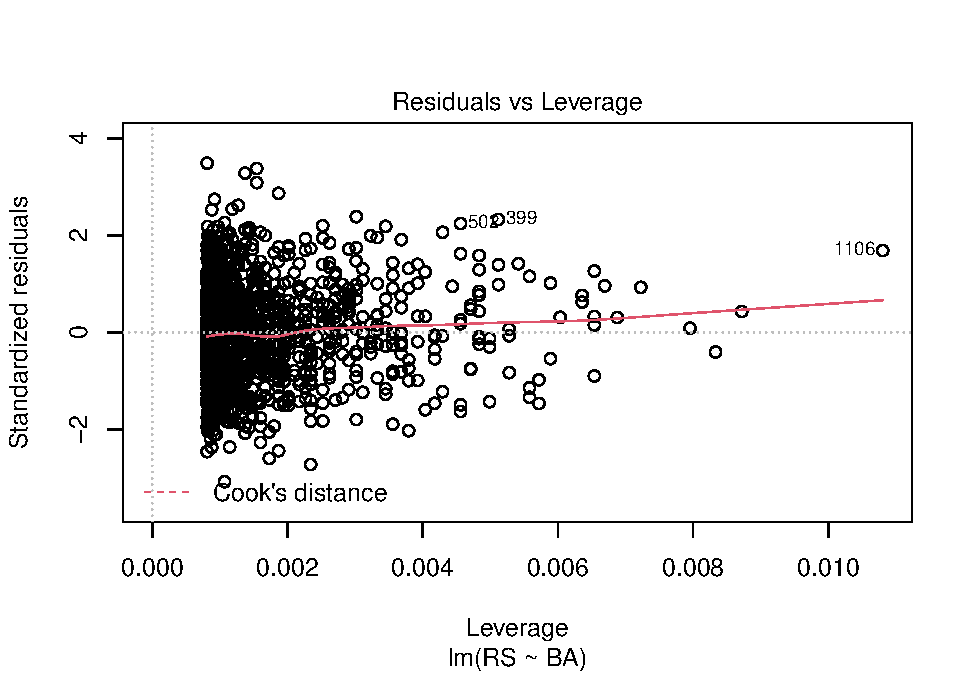
\includegraphics{HW2_Liu-Zi-Jian_files/figure-latex/unnamed-chunk-34-4.pdf}

From the second plot, the QQ plot of the fitted residuals for model RS
\textasciitilde{} BA, we can verify that the residuals are not skewly
distributed and that the model is reasonable.

\begin{Shaded}
\begin{Highlighting}[]
\NormalTok{OBPfit <-}\StringTok{ }\KeywordTok{lm}\NormalTok{(RS }\OperatorTok{~}\StringTok{ }\NormalTok{OBP, }\DataTypeTok{data =}\NormalTok{ baseballData)}
\KeywordTok{summary}\NormalTok{(OBPfit)}
\end{Highlighting}
\end{Shaded}

\begin{verbatim}
## 
## Call:
## lm(formula = RS ~ OBP, data = baseballData)
## 
## Residuals:
##      Min       1Q   Median       3Q      Max 
## -122.129  -27.110    1.284   26.441  135.265 
## 
## Coefficients:
##             Estimate Std. Error t value Pr(>|t|)    
## (Intercept)  -1076.6       24.7  -43.59   <2e-16 ***
## OBP           5490.4       75.6   72.62   <2e-16 ***
## ---
## Signif. codes:  0 '***' 0.001 '**' 0.01 '*' 0.05 '.' 0.1 ' ' 1
## 
## Residual standard error: 39.82 on 1230 degrees of freedom
## Multiple R-squared:  0.8109, Adjusted R-squared:  0.8107 
## F-statistic:  5274 on 1 and 1230 DF,  p-value: < 2.2e-16
\end{verbatim}

\begin{Shaded}
\begin{Highlighting}[]
\KeywordTok{plot}\NormalTok{(baseballData}\OperatorTok{$}\NormalTok{OBP, baseballData}\OperatorTok{$}\NormalTok{RS)}
\KeywordTok{abline}\NormalTok{(OBPfit)}
\end{Highlighting}
\end{Shaded}

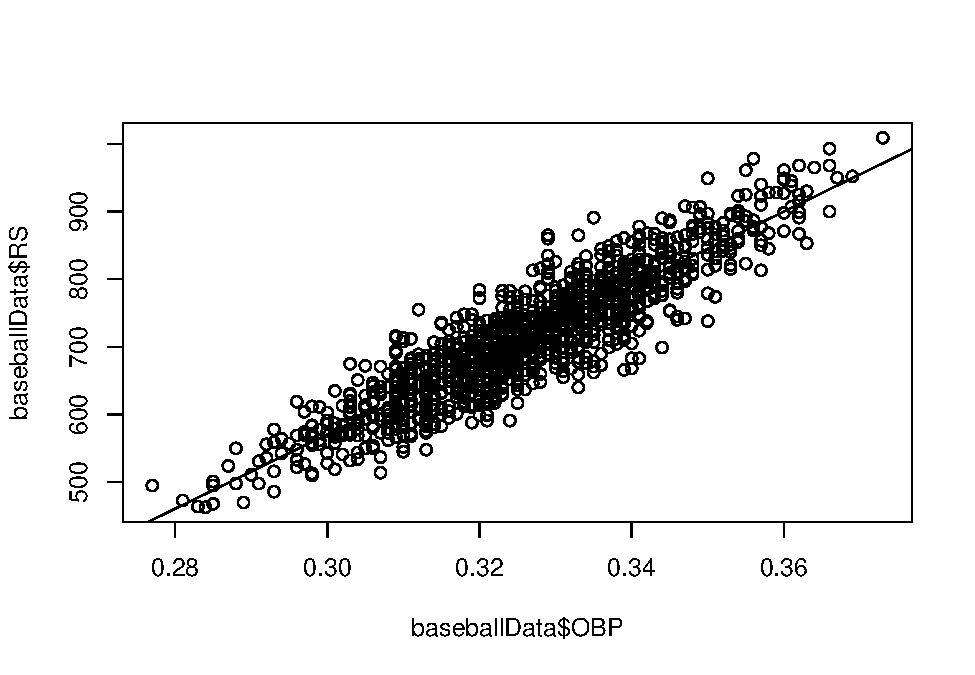
\includegraphics{HW2_Liu-Zi-Jian_files/figure-latex/unnamed-chunk-35-1.pdf}

Above is the scatter plot using model RS \textasciitilde{} OBP. The
intercept and slope are -1076.6, and 5490.4 respectively, the Rsquared
is 0.8109

\begin{Shaded}
\begin{Highlighting}[]
\KeywordTok{plot}\NormalTok{(OBPfit)}
\end{Highlighting}
\end{Shaded}

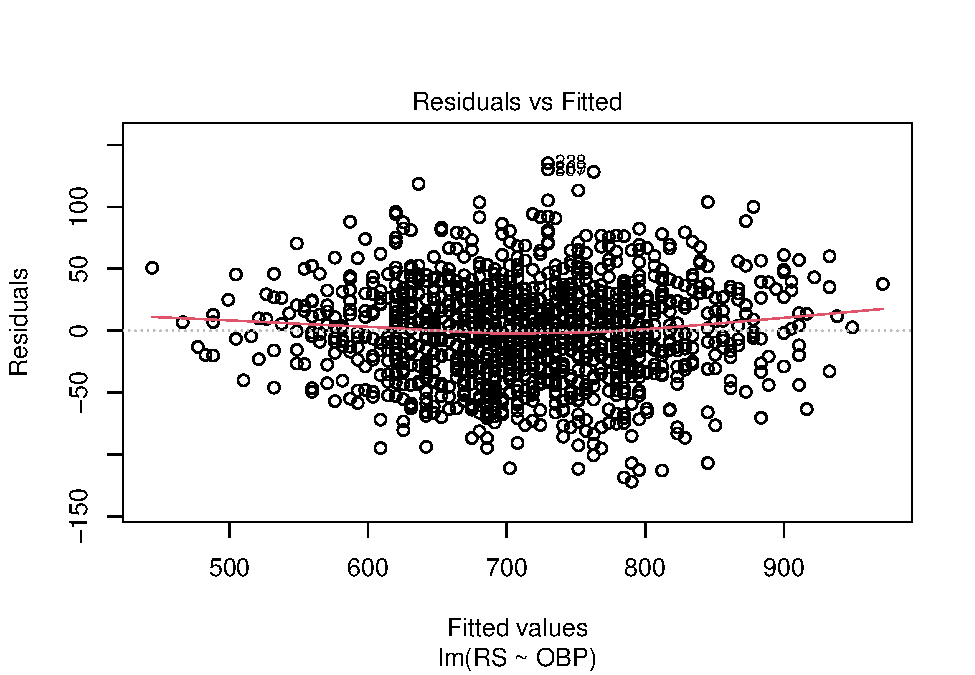
\includegraphics{HW2_Liu-Zi-Jian_files/figure-latex/unnamed-chunk-36-1.pdf}
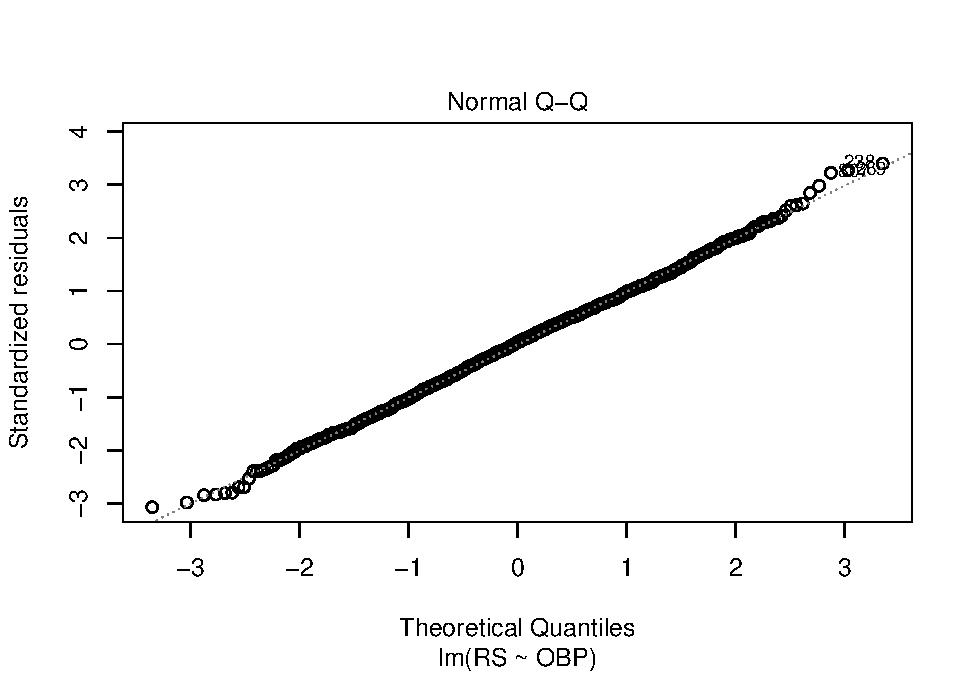
\includegraphics{HW2_Liu-Zi-Jian_files/figure-latex/unnamed-chunk-36-2.pdf}
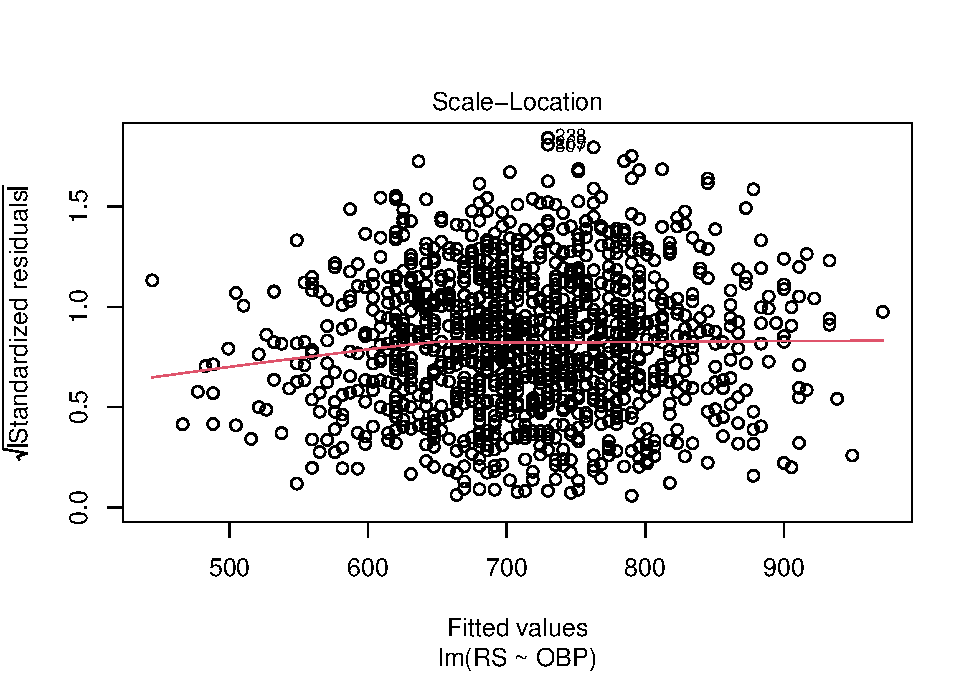
\includegraphics{HW2_Liu-Zi-Jian_files/figure-latex/unnamed-chunk-36-3.pdf}
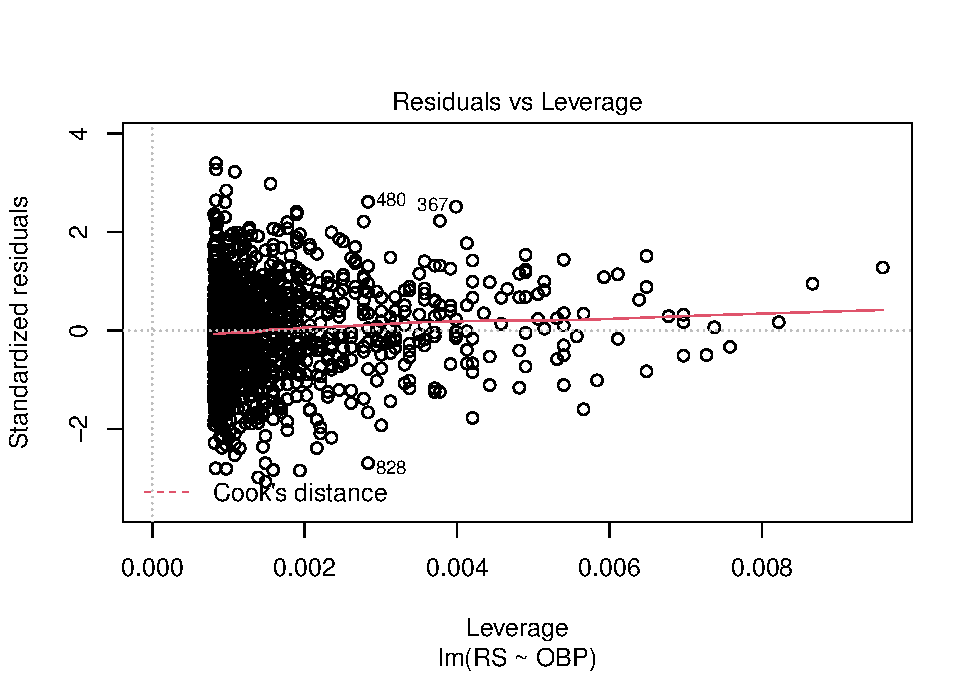
\includegraphics{HW2_Liu-Zi-Jian_files/figure-latex/unnamed-chunk-36-4.pdf}

From the second plot, the QQ plot of the fitted residuals for model RS
\textasciitilde{} OBP, we can verify that the residuals are not skewly
distributed and that the model is reasonable.

\begin{Shaded}
\begin{Highlighting}[]
\NormalTok{SLGfit <-}\StringTok{ }\KeywordTok{lm}\NormalTok{(RS }\OperatorTok{~}\StringTok{ }\NormalTok{SLG, }\DataTypeTok{data =}\NormalTok{ baseballData)}
\KeywordTok{summary}\NormalTok{(SLGfit)}
\end{Highlighting}
\end{Shaded}

\begin{verbatim}
## 
## Call:
## lm(formula = RS ~ SLG, data = baseballData)
## 
## Residuals:
##      Min       1Q   Median       3Q      Max 
## -119.919  -23.666   -1.541   22.353  131.812 
## 
## Coefficients:
##             Estimate Std. Error t value Pr(>|t|)    
## (Intercept)  -289.37      12.35  -23.43   <2e-16 ***
## SLG          2527.92      30.98   81.60   <2e-16 ***
## ---
## Signif. codes:  0 '***' 0.001 '**' 0.01 '*' 0.05 '.' 0.1 ' ' 1
## 
## Residual standard error: 36.16 on 1230 degrees of freedom
## Multiple R-squared:  0.8441, Adjusted R-squared:  0.844 
## F-statistic:  6659 on 1 and 1230 DF,  p-value: < 2.2e-16
\end{verbatim}

\begin{Shaded}
\begin{Highlighting}[]
\KeywordTok{plot}\NormalTok{(baseballData}\OperatorTok{$}\NormalTok{SLG, baseballData}\OperatorTok{$}\NormalTok{RS)}
\KeywordTok{abline}\NormalTok{(SLGfit)}
\end{Highlighting}
\end{Shaded}

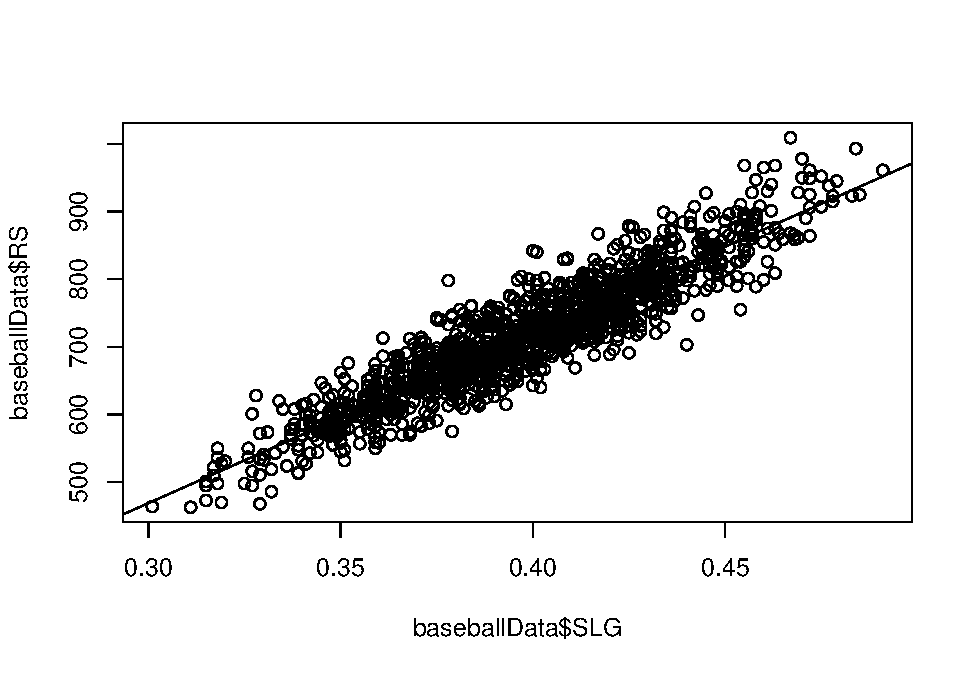
\includegraphics{HW2_Liu-Zi-Jian_files/figure-latex/unnamed-chunk-37-1.pdf}

Above is the scatter plot using model RS \textasciitilde{} SLG. The
intercept and slope are -289.37, and 2527.92 respectively, the Rsquared
is 0.8441

\begin{Shaded}
\begin{Highlighting}[]
\KeywordTok{plot}\NormalTok{(SLGfit)}
\end{Highlighting}
\end{Shaded}

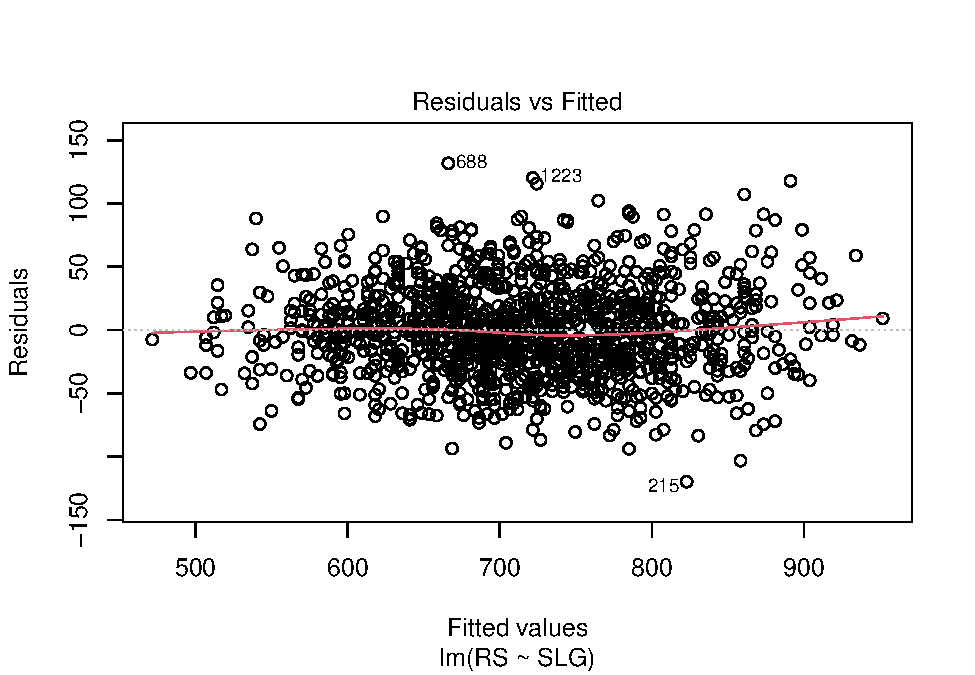
\includegraphics{HW2_Liu-Zi-Jian_files/figure-latex/unnamed-chunk-38-1.pdf}
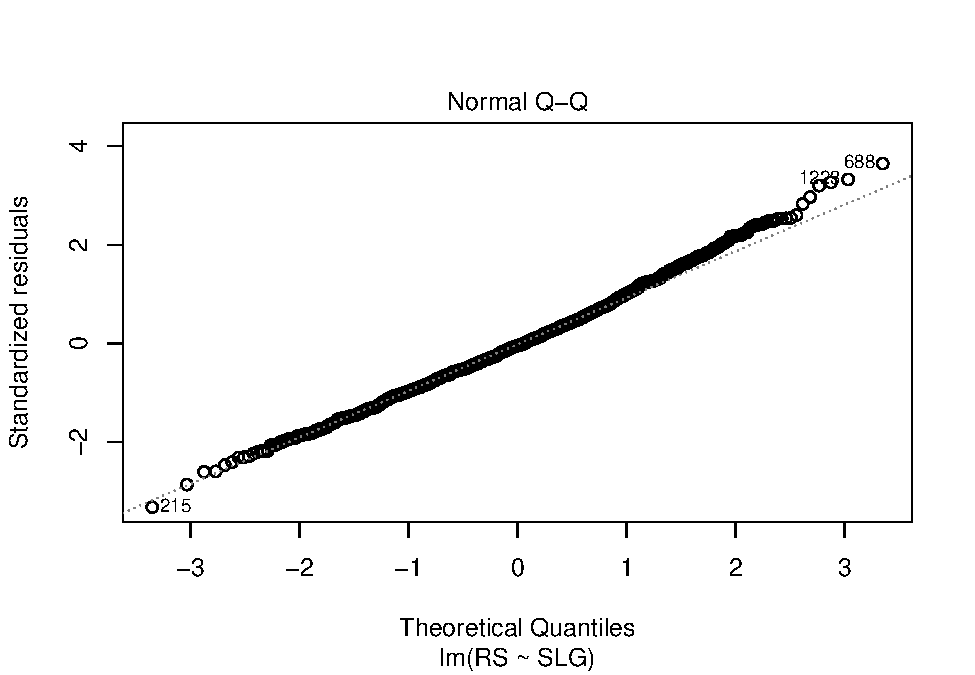
\includegraphics{HW2_Liu-Zi-Jian_files/figure-latex/unnamed-chunk-38-2.pdf}
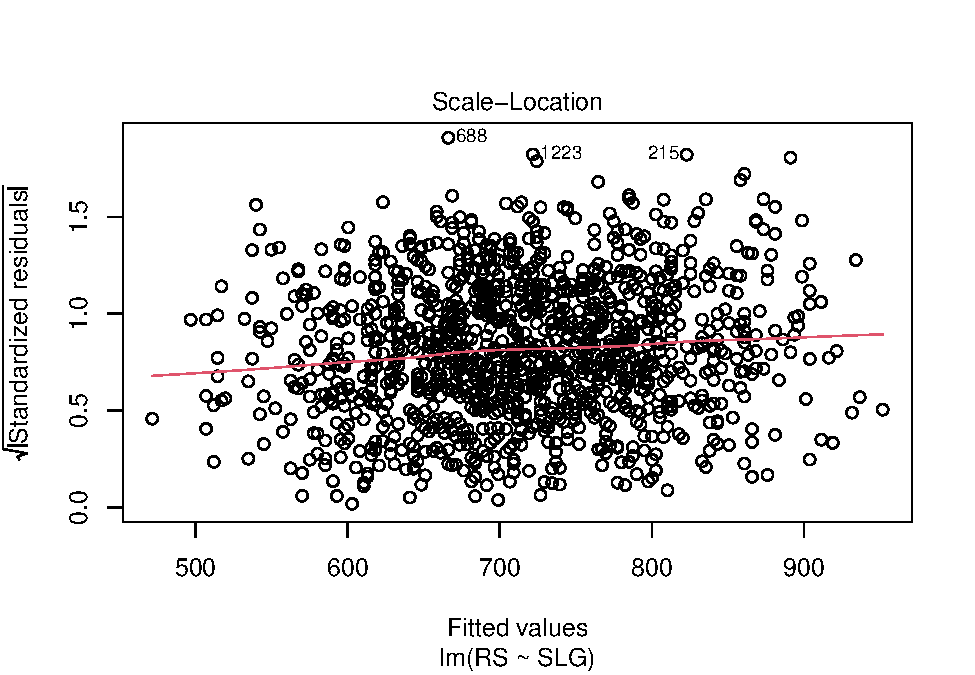
\includegraphics{HW2_Liu-Zi-Jian_files/figure-latex/unnamed-chunk-38-3.pdf}
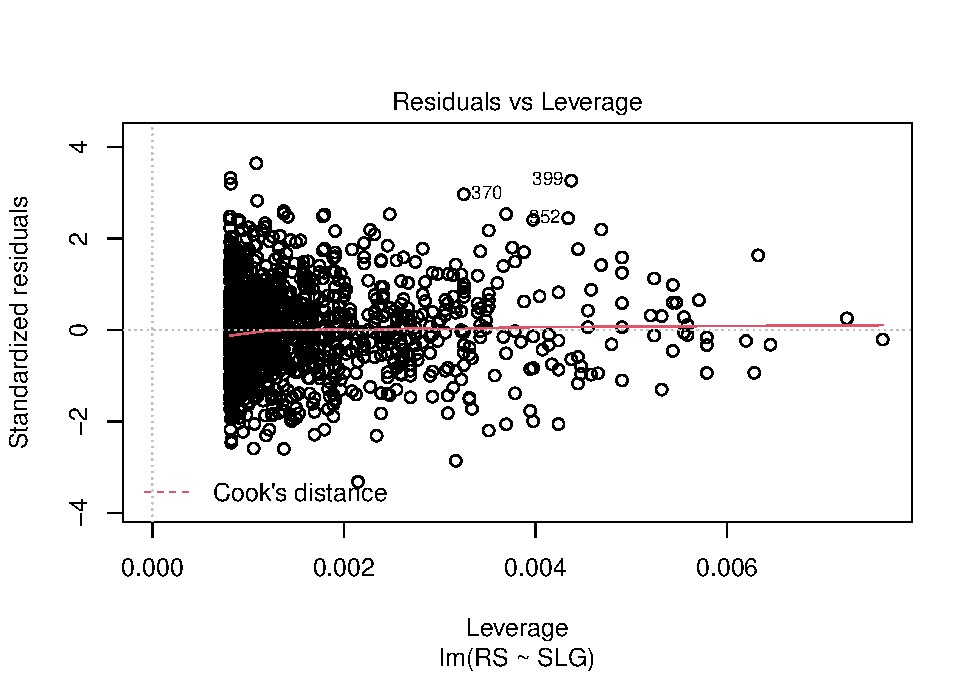
\includegraphics{HW2_Liu-Zi-Jian_files/figure-latex/unnamed-chunk-38-4.pdf}

From the second plot, the QQ plot of the fitted residuals for model RS
\textasciitilde{} SLG, we can verify that the residuals are not skewly
distributed and that the model is reasonable.

Comparing the Rsquared results, we see that Rsquared for BA = 0.6839,
Rsquared for OBP = 0.8109 and Rsquared for SLG = 0.8441. We see that the
Rsquared result for OBP and for SLG is higher than the Rsquared for BA.
That is consistent with Billy's claim that OBP and SLG have much more
impact than BA. This is not consistent with the intuition that BA is
thought to be the most responsible for RS.

\hypertarget{part-iii.-multiple-regression-analysis-1}{%
\subsection{4. Part III. Multiple Regression
Analysis}\label{part-iii.-multiple-regression-analysis-1}}

\begin{Shaded}
\begin{Highlighting}[]
\NormalTok{multi_fitBaseball =}\StringTok{ }\KeywordTok{lm}\NormalTok{(RS }\OperatorTok{~}\StringTok{ }\NormalTok{BA }\OperatorTok{+}\StringTok{ }\NormalTok{SLG }\OperatorTok{+}\StringTok{ }\NormalTok{OBP, }\DataTypeTok{data =}\NormalTok{ baseballData)}
\KeywordTok{summary}\NormalTok{(multi_fitBaseball)}
\end{Highlighting}
\end{Shaded}

\begin{verbatim}
## 
## Call:
## lm(formula = RS ~ BA + SLG + OBP, data = baseballData)
## 
## Residuals:
##     Min      1Q  Median      3Q     Max 
## -79.693 -16.667  -0.892  16.556  93.068 
## 
## Coefficients:
##             Estimate Std. Error t value Pr(>|t|)    
## (Intercept)  -806.08      17.39 -46.348   <2e-16 ***
## BA           -134.90     113.73  -1.186    0.236    
## SLG          1533.88      37.76  40.623   <2e-16 ***
## OBP          2900.94      97.87  29.640   <2e-16 ***
## ---
## Signif. codes:  0 '***' 0.001 '**' 0.01 '*' 0.05 '.' 0.1 ' ' 1
## 
## Residual standard error: 25.12 on 1228 degrees of freedom
## Multiple R-squared:  0.9249, Adjusted R-squared:  0.9247 
## F-statistic:  5040 on 3 and 1228 DF,  p-value: < 2.2e-16
\end{verbatim}

\begin{Shaded}
\begin{Highlighting}[]
\KeywordTok{plot}\NormalTok{(multi_fitBaseball)}
\end{Highlighting}
\end{Shaded}

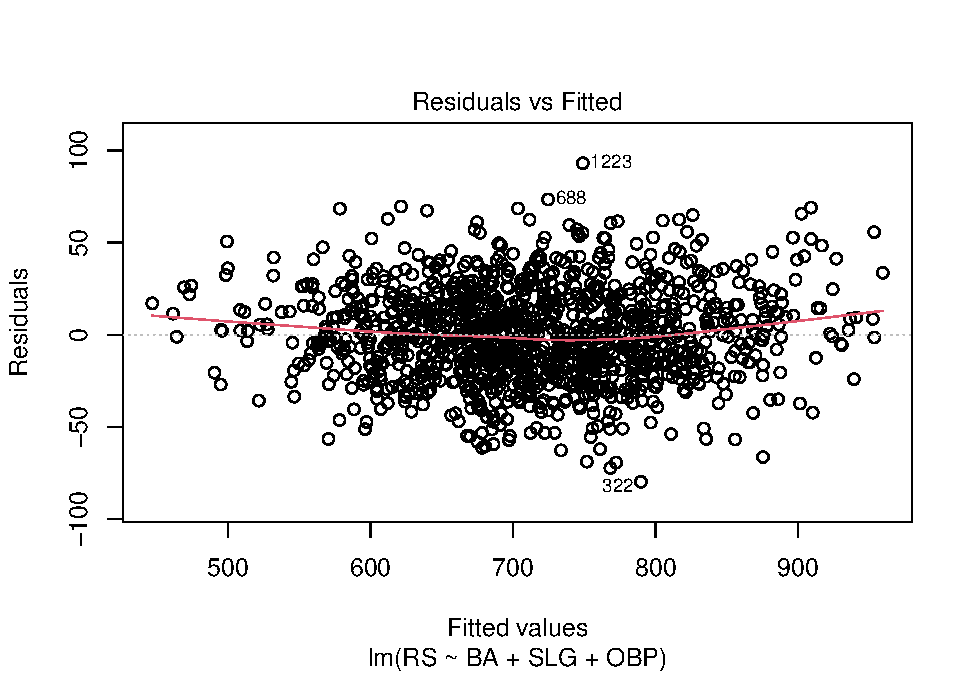
\includegraphics{HW2_Liu-Zi-Jian_files/figure-latex/unnamed-chunk-39-1.pdf}
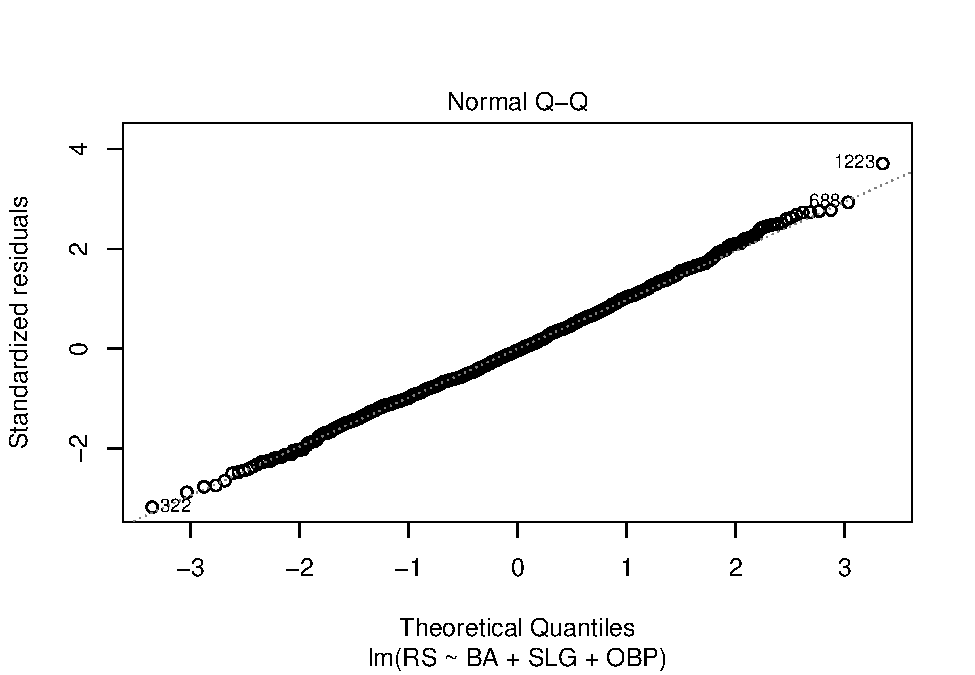
\includegraphics{HW2_Liu-Zi-Jian_files/figure-latex/unnamed-chunk-39-2.pdf}
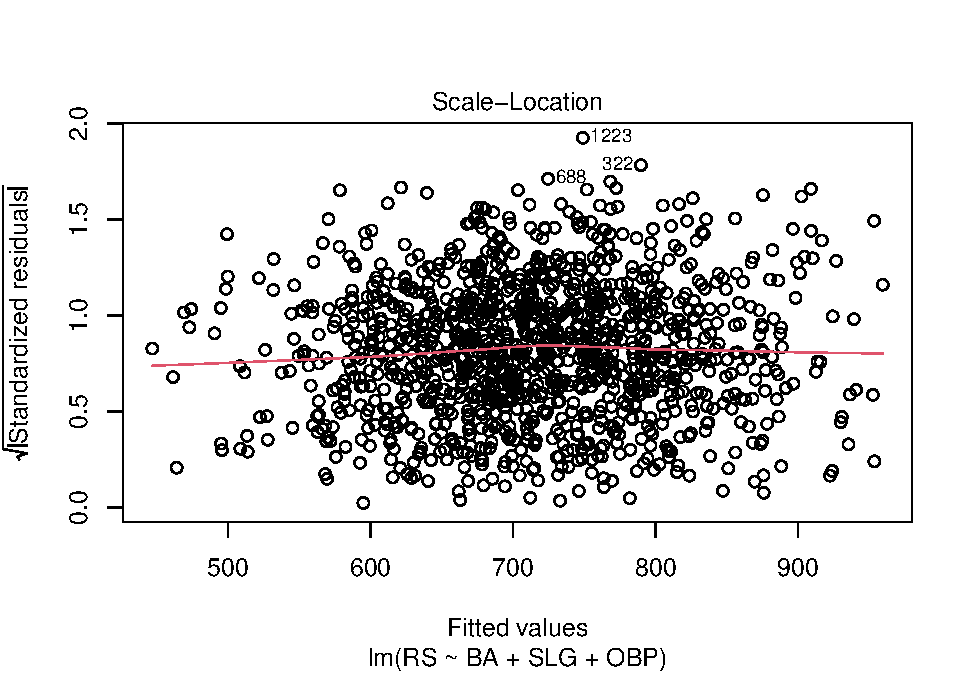
\includegraphics{HW2_Liu-Zi-Jian_files/figure-latex/unnamed-chunk-39-3.pdf}
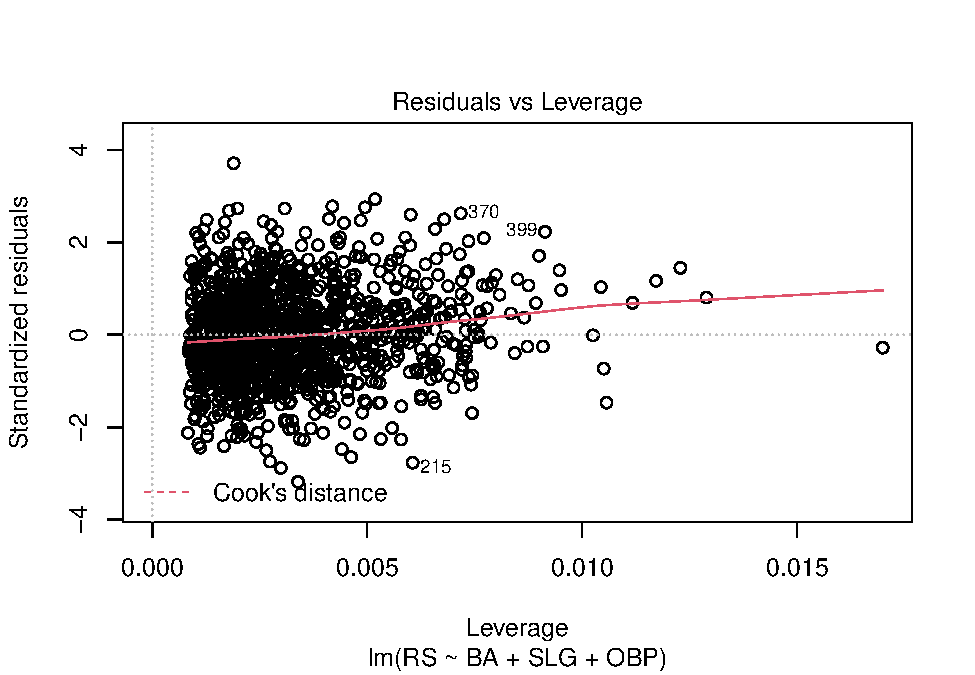
\includegraphics{HW2_Liu-Zi-Jian_files/figure-latex/unnamed-chunk-39-4.pdf}

For the model RS ∼ BA + SLG + OBP, the intercept is -806.08, and the
coefficient for BA is -134.90 with significance p = 0.236 the
coefficient for SLG is 1533.88 with significance p \textless{} 2e-16 And
the coefficient for OBP is 2900.94 with significance p \textless{}
2e-16. The second plot above is the QQ plot of the residuals. We can
verify that the residuals are not skewly distributed and that the model
is reasonable. The fitting results is not consistent with that in Part
II, especially for the fitted coefficient of BA. (coeff = 5864.84 vs
-134.90, one is a big positive, and the other is negative). We find that
BA is not significant and SLG and OBP is significant

\begin{Shaded}
\begin{Highlighting}[]
\NormalTok{multi_fitBaseball2 =}\StringTok{ }\KeywordTok{lm}\NormalTok{(RS }\OperatorTok{~}\StringTok{ }\NormalTok{BA }\OperatorTok{+}\StringTok{ }\NormalTok{SLG, }\DataTypeTok{data =}\NormalTok{ baseballData)}
\KeywordTok{summary}\NormalTok{(multi_fitBaseball2)}
\end{Highlighting}
\end{Shaded}

\begin{verbatim}
## 
## Call:
## lm(formula = RS ~ BA + SLG, data = baseballData)
## 
## Residuals:
##      Min       1Q   Median       3Q      Max 
## -115.432  -23.284   -2.048   21.068  113.415 
## 
## Coefficients:
##             Estimate Std. Error t value Pr(>|t|)    
## (Intercept)  -551.08      19.79  -27.85   <2e-16 ***
## BA           1904.66     118.56   16.07   <2e-16 ***
## SLG          1943.77      46.00   42.26   <2e-16 ***
## ---
## Signif. codes:  0 '***' 0.001 '**' 0.01 '*' 0.05 '.' 0.1 ' ' 1
## 
## Residual standard error: 32.88 on 1229 degrees of freedom
## Multiple R-squared:  0.8711, Adjusted R-squared:  0.8709 
## F-statistic:  4154 on 2 and 1229 DF,  p-value: < 2.2e-16
\end{verbatim}

\begin{Shaded}
\begin{Highlighting}[]
\KeywordTok{plot}\NormalTok{(multi_fitBaseball2)}
\end{Highlighting}
\end{Shaded}

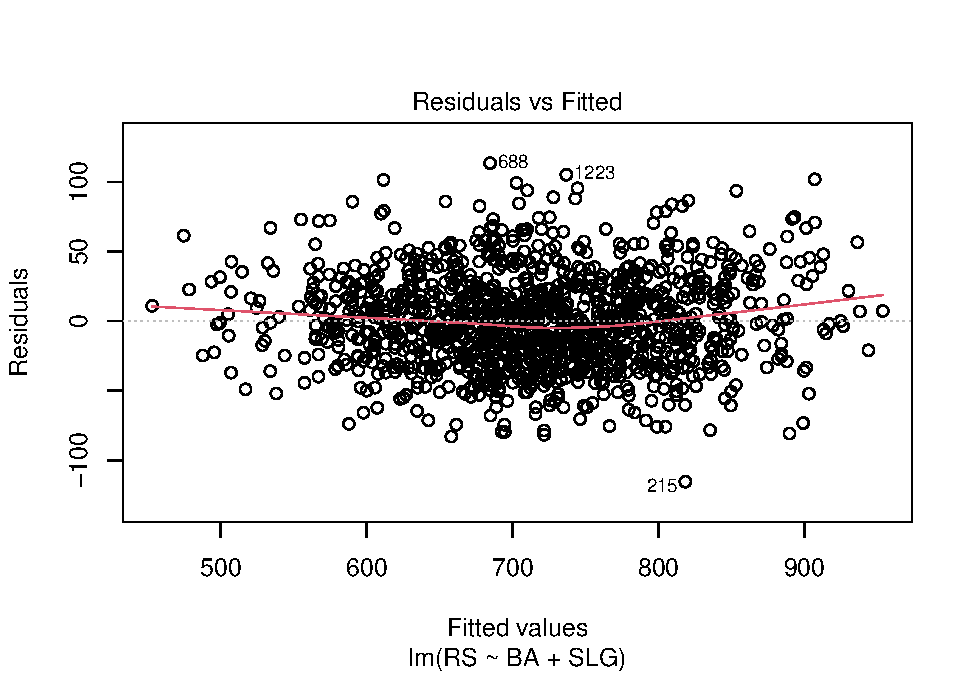
\includegraphics{HW2_Liu-Zi-Jian_files/figure-latex/unnamed-chunk-40-1.pdf}
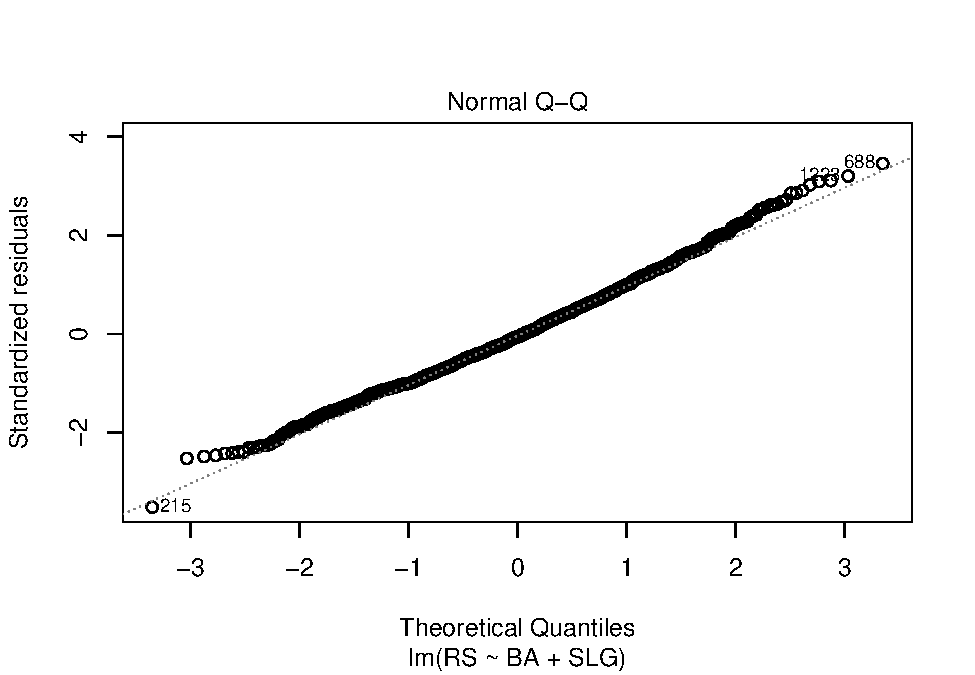
\includegraphics{HW2_Liu-Zi-Jian_files/figure-latex/unnamed-chunk-40-2.pdf}
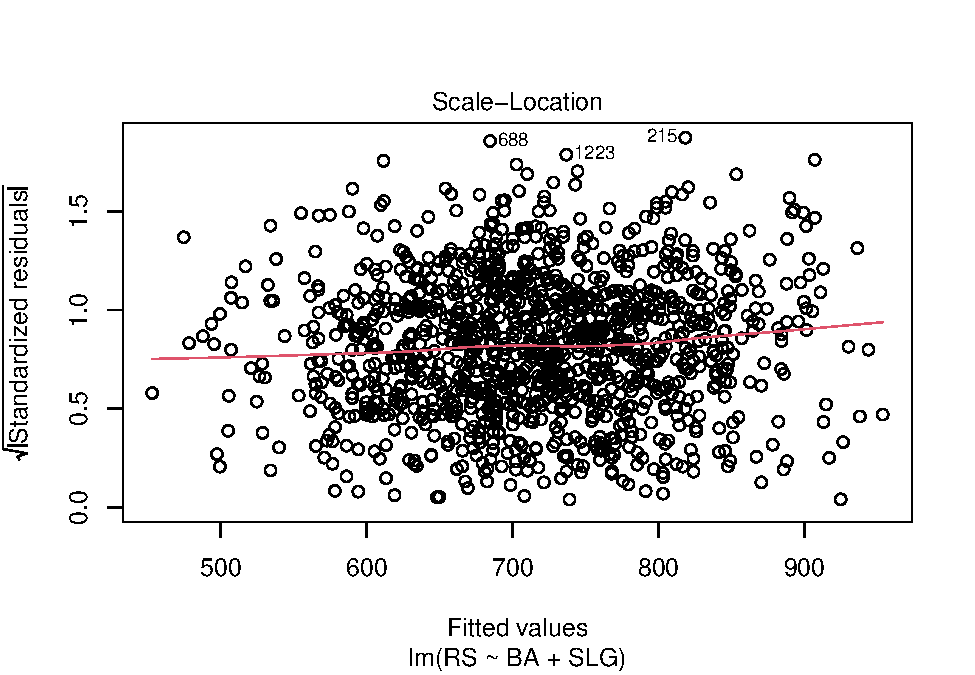
\includegraphics{HW2_Liu-Zi-Jian_files/figure-latex/unnamed-chunk-40-3.pdf}
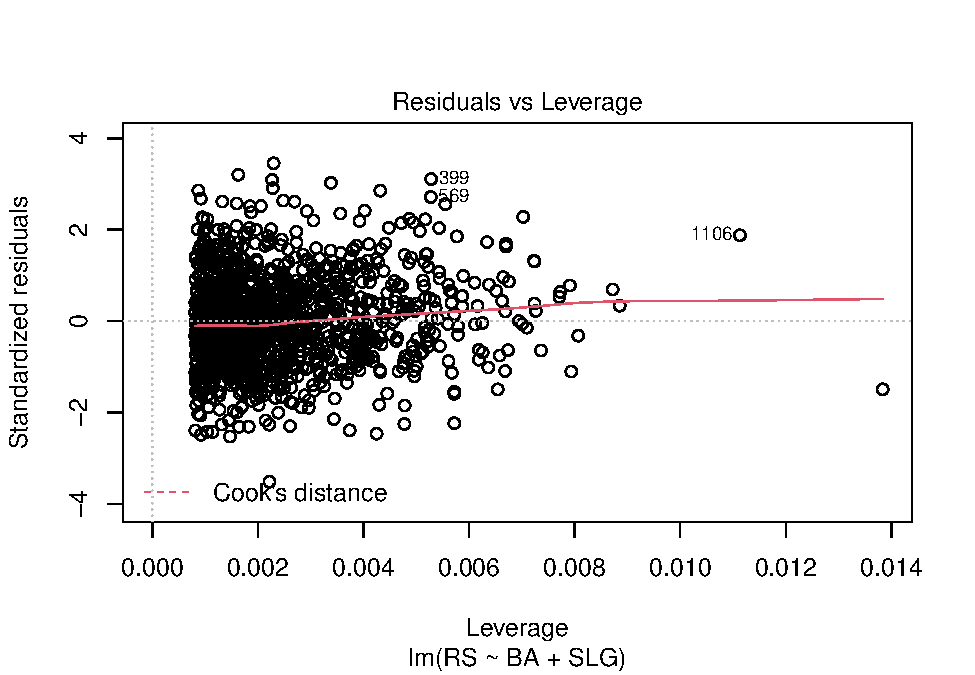
\includegraphics{HW2_Liu-Zi-Jian_files/figure-latex/unnamed-chunk-40-4.pdf}

For the model RS ∼ BA + SLG , the intercept is -551.08, and the
coefficient for BA is 1904.66 with significance p \textless{} 2e-16 the
coefficient for SLG is 1943.77 with significance p \textless{} 2e-16.
The second plot above is the QQ plot of the residuals. We can verify
that the residuals are not skewly distributed and that the model is
reasonable. The fitting results is more consistent with that in Part II,
especially for the fitted coefficient of BA. (coeff = 5864.84 vs 1904.66
vs -134.90 for model RS ∼ BA + SLG + OBP). Both of these variables are
significant.

Comparing the Rsquared for both of these models: for model RS ∼ BA + SLG
+ OBP, Rsquared = 0.9249, and for model RS ∼ BA + SLG, Rsquared =
0.8711. Therefore the model that we prefer is RS ∼ BA + SLG + OBP since
the Rsquared is greater.

So in the question they want RS ∼ BA + SLG. However we want to remove BA
so here is an extra regression for model RS \textasciitilde{} SLG + OBP

\begin{Shaded}
\begin{Highlighting}[]
\NormalTok{multi_fitBaseball3 =}\StringTok{ }\KeywordTok{lm}\NormalTok{(RS }\OperatorTok{~}\StringTok{ }\NormalTok{SLG }\OperatorTok{+}\StringTok{ }\NormalTok{OBP, }\DataTypeTok{data =}\NormalTok{ baseballData)}
\KeywordTok{summary}\NormalTok{(multi_fitBaseball3)}
\end{Highlighting}
\end{Shaded}

\begin{verbatim}
## 
## Call:
## lm(formula = RS ~ SLG + OBP, data = baseballData)
## 
## Residuals:
##     Min      1Q  Median      3Q     Max 
## -78.365 -16.821  -1.208  16.477  92.684 
## 
## Coefficients:
##             Estimate Std. Error t value Pr(>|t|)    
## (Intercept)  -811.66      16.75  -48.47   <2e-16 ***
## SLG          1517.58      35.17   43.15   <2e-16 ***
## OBP          2830.70      77.94   36.32   <2e-16 ***
## ---
## Signif. codes:  0 '***' 0.001 '**' 0.01 '*' 0.05 '.' 0.1 ' ' 1
## 
## Residual standard error: 25.12 on 1229 degrees of freedom
## Multiple R-squared:  0.9248, Adjusted R-squared:  0.9247 
## F-statistic:  7557 on 2 and 1229 DF,  p-value: < 2.2e-16
\end{verbatim}

\begin{Shaded}
\begin{Highlighting}[]
\KeywordTok{plot}\NormalTok{(multi_fitBaseball3)}
\end{Highlighting}
\end{Shaded}

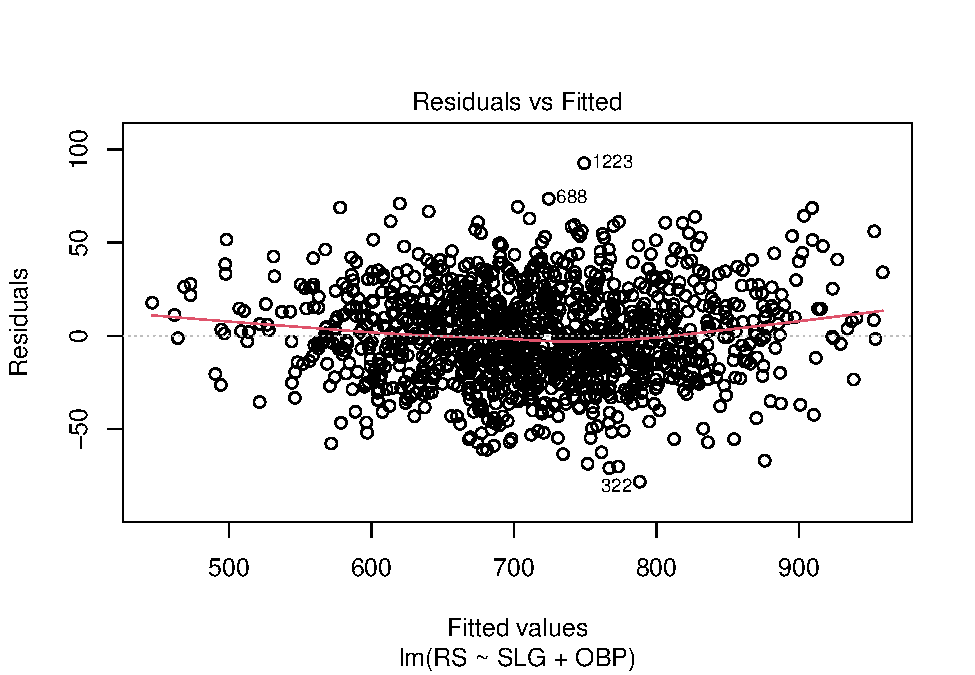
\includegraphics{HW2_Liu-Zi-Jian_files/figure-latex/unnamed-chunk-41-1.pdf}
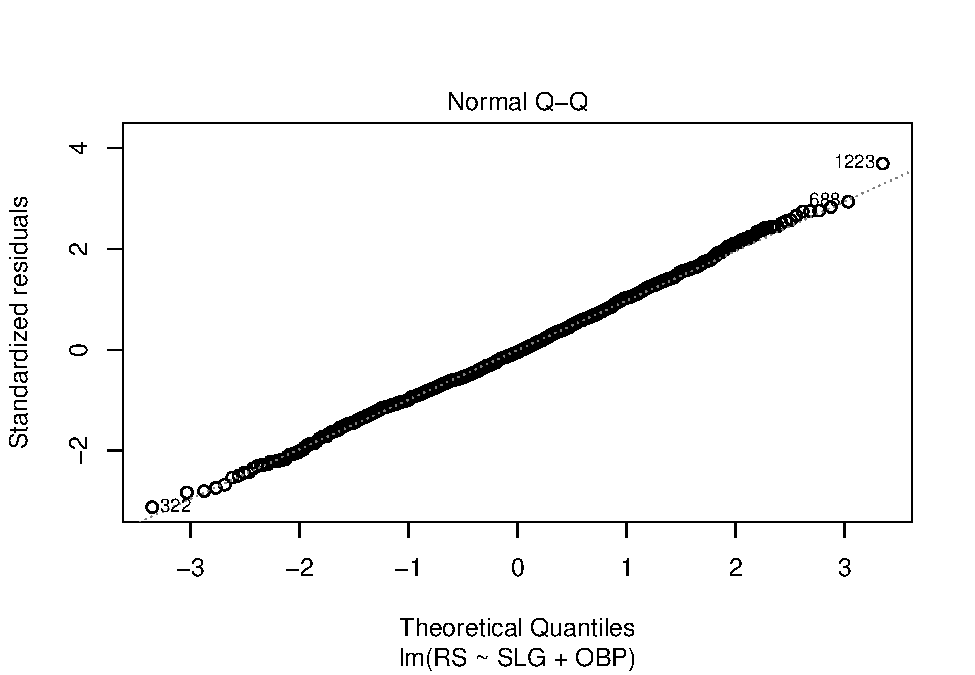
\includegraphics{HW2_Liu-Zi-Jian_files/figure-latex/unnamed-chunk-41-2.pdf}
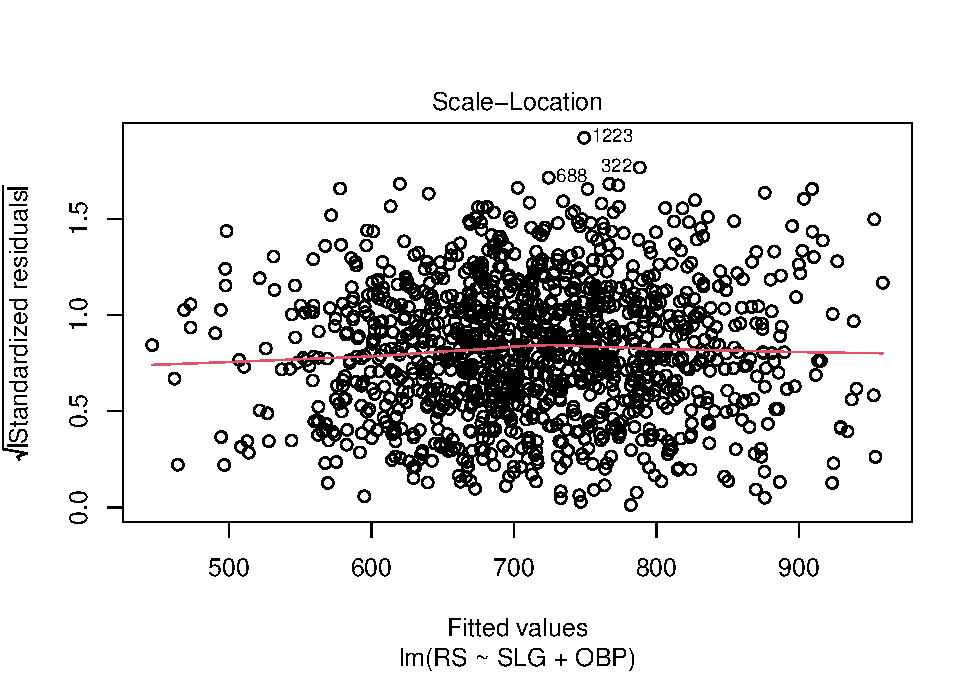
\includegraphics{HW2_Liu-Zi-Jian_files/figure-latex/unnamed-chunk-41-3.pdf}
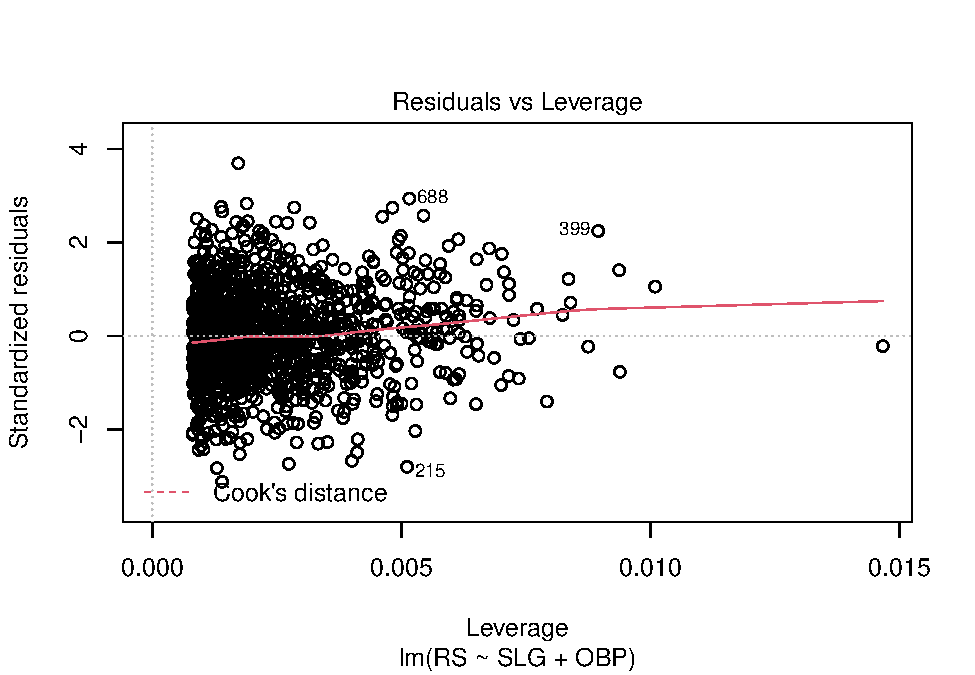
\includegraphics{HW2_Liu-Zi-Jian_files/figure-latex/unnamed-chunk-41-4.pdf}

For the model RS ∼ SLG + OBP , the intercept is -811.66, and the
coefficient for SLG is 1517.58 with significance p \textless{} 2e-16 the
coefficient for OBP is 2830.70 with significance p \textless{} 2e-16.
The second plot above is the QQ plot of the residuals. We can verify
that the residuals are not skewly distributed and that the model is
reasonable. Both of these variables are significant.

Comparing the Rsquared for models: for model RS ∼ BA + SLG + OBP,
Rsquared = 0.9249, and for model RS ∼ SLG + OBP, Rsquared = 0.9248. Both
Rsquared is roughly the same so we can consider dropping BA and just
have SLG and OBP in our model.

\hypertarget{part-iv.}{%
\subsection{4. Part IV.}\label{part-iv.}}

\begin{Shaded}
\begin{Highlighting}[]
\KeywordTok{head}\NormalTok{(baseballData)}
\end{Highlighting}
\end{Shaded}

\begin{verbatim}
##   Team League Year  RS  RA  W   OBP   SLG    BA Playoffs RankSeason
## 1  ARI     NL 2012 734 688 81 0.328 0.418 0.259        0         NA
## 2  ATL     NL 2012 700 600 94 0.320 0.389 0.247        1          4
## 3  BAL     AL 2012 712 705 93 0.311 0.417 0.247        1          5
## 4  BOS     AL 2012 734 806 69 0.315 0.415 0.260        0         NA
## 5  CHC     NL 2012 613 759 61 0.302 0.378 0.240        0         NA
## 6  CHW     AL 2012 748 676 85 0.318 0.422 0.255        0         NA
##   RankPlayoffs   G  OOBP  OSLG
## 1           NA 162 0.317 0.415
## 2            5 162 0.306 0.378
## 3            4 162 0.315 0.403
## 4           NA 162 0.331 0.428
## 5           NA 162 0.335 0.424
## 6           NA 162 0.319 0.405
\end{verbatim}

\begin{Shaded}
\begin{Highlighting}[]
\NormalTok{RD <-}\StringTok{ }\NormalTok{baseballData}\OperatorTok{$}\NormalTok{RS }\OperatorTok{-}\StringTok{ }\NormalTok{baseballData}\OperatorTok{$}\NormalTok{RA}
\NormalTok{baseballData2 <-}\StringTok{ }\NormalTok{baseballData}
\NormalTok{baseballData2}\OperatorTok{$}\NormalTok{RD=RD}
\NormalTok{baseballData2 <-}\StringTok{ }\NormalTok{baseballData2[baseballData2}\OperatorTok{$}\NormalTok{Year }\OperatorTok{<}\StringTok{ }\DecValTok{2002}\NormalTok{, ]}
\KeywordTok{head}\NormalTok{(baseballData2)}
\end{Highlighting}
\end{Shaded}

\begin{verbatim}
##     Team League Year  RS  RA  W   OBP   SLG    BA Playoffs RankSeason
## 331  ANA     AL 2001 691 730 75 0.327 0.405 0.261        0         NA
## 332  ARI     NL 2001 818 677 92 0.341 0.442 0.267        1          5
## 333  ATL     NL 2001 729 643 88 0.324 0.412 0.260        1          7
## 334  BAL     AL 2001 687 829 63 0.319 0.380 0.248        0         NA
## 335  BOS     AL 2001 772 745 82 0.334 0.439 0.266        0         NA
## 336  CHC     NL 2001 777 701 88 0.336 0.430 0.261        0         NA
##     RankPlayoffs   G  OOBP  OSLG   RD
## 331           NA 162 0.331 0.412  -39
## 332            1 162 0.311 0.404  141
## 333            3 162 0.314 0.384   86
## 334           NA 162 0.337 0.439 -142
## 335           NA 161 0.329 0.393   27
## 336           NA 162 0.321 0.398   76
\end{verbatim}

\begin{Shaded}
\begin{Highlighting}[]
\NormalTok{modelw_rd =}\StringTok{ }\KeywordTok{lm}\NormalTok{(W }\OperatorTok{~}\StringTok{ }\NormalTok{RD, }\DataTypeTok{data =}\NormalTok{ baseballData2)}
\KeywordTok{summary}\NormalTok{(modelw_rd)}
\end{Highlighting}
\end{Shaded}

\begin{verbatim}
## 
## Call:
## lm(formula = W ~ RD, data = baseballData2)
## 
## Residuals:
##      Min       1Q   Median       3Q      Max 
## -14.2662  -2.6509   0.1234   2.9364  11.6570 
## 
## Coefficients:
##              Estimate Std. Error t value Pr(>|t|)    
## (Intercept) 80.881375   0.131157  616.67   <2e-16 ***
## RD           0.105766   0.001297   81.55   <2e-16 ***
## ---
## Signif. codes:  0 '***' 0.001 '**' 0.01 '*' 0.05 '.' 0.1 ' ' 1
## 
## Residual standard error: 3.939 on 900 degrees of freedom
## Multiple R-squared:  0.8808, Adjusted R-squared:  0.8807 
## F-statistic:  6651 on 1 and 900 DF,  p-value: < 2.2e-16
\end{verbatim}

\begin{Shaded}
\begin{Highlighting}[]
\NormalTok{modelrs =}\StringTok{ }\KeywordTok{lm}\NormalTok{(RS }\OperatorTok{~}\StringTok{ }\NormalTok{OBP }\OperatorTok{+}\StringTok{ }\NormalTok{SLG, }\DataTypeTok{data =}\NormalTok{ baseballData2)}
\KeywordTok{summary}\NormalTok{(modelrs)}
\end{Highlighting}
\end{Shaded}

\begin{verbatim}
## 
## Call:
## lm(formula = RS ~ OBP + SLG, data = baseballData2)
## 
## Residuals:
##     Min      1Q  Median      3Q     Max 
## -70.838 -17.174  -1.108  16.770  90.036 
## 
## Coefficients:
##             Estimate Std. Error t value Pr(>|t|)    
## (Intercept)  -804.63      18.92  -42.53   <2e-16 ***
## OBP          2737.77      90.68   30.19   <2e-16 ***
## SLG          1584.91      42.16   37.60   <2e-16 ***
## ---
## Signif. codes:  0 '***' 0.001 '**' 0.01 '*' 0.05 '.' 0.1 ' ' 1
## 
## Residual standard error: 24.79 on 899 degrees of freedom
## Multiple R-squared:  0.9296, Adjusted R-squared:  0.9294 
## F-statistic:  5934 on 2 and 899 DF,  p-value: < 2.2e-16
\end{verbatim}

\begin{Shaded}
\begin{Highlighting}[]
\NormalTok{modelra =}\StringTok{ }\KeywordTok{lm}\NormalTok{(RA }\OperatorTok{~}\StringTok{ }\NormalTok{OOBP }\OperatorTok{+}\StringTok{ }\NormalTok{OSLG, }\DataTypeTok{data =}\NormalTok{ baseballData2)}
\KeywordTok{summary}\NormalTok{(modelra)}
\end{Highlighting}
\end{Shaded}

\begin{verbatim}
## 
## Call:
## lm(formula = RA ~ OOBP + OSLG, data = baseballData2)
## 
## Residuals:
##     Min      1Q  Median      3Q     Max 
## -82.397 -15.178  -0.129  17.679  60.955 
## 
## Coefficients:
##             Estimate Std. Error t value Pr(>|t|)    
## (Intercept)  -837.38      60.26 -13.897  < 2e-16 ***
## OOBP         2913.60     291.97   9.979 4.46e-16 ***
## OSLG         1514.29     175.43   8.632 2.55e-13 ***
## ---
## Signif. codes:  0 '***' 0.001 '**' 0.01 '*' 0.05 '.' 0.1 ' ' 1
## 
## Residual standard error: 25.67 on 87 degrees of freedom
##   (812 observations deleted due to missingness)
## Multiple R-squared:  0.9073, Adjusted R-squared:  0.9052 
## F-statistic: 425.8 on 2 and 87 DF,  p-value: < 2.2e-16
\end{verbatim}

in 2002 OBP = .349, SLG = .430, OOBP = .307 and OSLG = .373 for Oakland
Athletics. we have that RA = -837.38 +2913.60xOOBP + 1514.29xOSLG RS =
-804.63 + 2737.77xOBP + 1584.91xSLG W = 80.881375 + 0.105766xRD

\begin{Shaded}
\begin{Highlighting}[]
\NormalTok{OBP =}\StringTok{ }\FloatTok{.349}
\NormalTok{SLG =}\StringTok{ }\FloatTok{.430}
\NormalTok{OOBP =}\StringTok{ }\FloatTok{.307}
\NormalTok{OSLG =}\StringTok{ }\FloatTok{.373}
\NormalTok{RA =}\StringTok{ }\FloatTok{-837.38} \FloatTok{+2913.60}\OperatorTok{*}\NormalTok{OOBP }\OperatorTok{+}\StringTok{ }\FloatTok{1514.29}\OperatorTok{*}\NormalTok{OSLG}
\NormalTok{RS =}\StringTok{ }\FloatTok{-804.63} \OperatorTok{+}\StringTok{ }\FloatTok{2737.77}\OperatorTok{*}\NormalTok{OBP }\OperatorTok{+}\StringTok{ }\FloatTok{1584.91}\OperatorTok{*}\NormalTok{SLG}
\NormalTok{RD =}\StringTok{ }\NormalTok{RS}\OperatorTok{-}\NormalTok{RA}
\NormalTok{W =}\StringTok{ }\FloatTok{80.881375} \OperatorTok{+}\StringTok{ }\FloatTok{0.105766}\OperatorTok{*}\NormalTok{RD}
\NormalTok{W}
\end{Highlighting}
\end{Shaded}

\begin{verbatim}
## [1] 103.1385
\end{verbatim}

From the three models, we can predict that Oakland would win 103 games
in 2002. By looking at our dataset, we see that Oakland did win 103
games in 2002

\begin{Shaded}
\begin{Highlighting}[]
\NormalTok{oakland <-}\StringTok{ }\NormalTok{baseballData}
\NormalTok{oakland[oakland}\OperatorTok{$}\NormalTok{Year }\OperatorTok{==}\StringTok{ }\DecValTok{2002} \OperatorTok{&}\StringTok{ }\NormalTok{oakland}\OperatorTok{$}\NormalTok{Team }\OperatorTok{==}\StringTok{ 'OAK'}\NormalTok{, ]}
\end{Highlighting}
\end{Shaded}

\begin{verbatim}
##     Team League Year  RS  RA   W   OBP   SLG    BA Playoffs RankSeason
## 321  OAK     AL 2002 800 654 103 0.339 0.432 0.261        1          1
##     RankPlayoffs   G  OOBP  OSLG
## 321            4 162 0.315 0.384
\end{verbatim}

\end{document}
